\documentclass[master,oneside,euler,openright,macfonts]{ustcthesis}
% 默认twoside 双面打印
% 将master修改为bachelor, doctor or master
% 要使用adobe字体,添加adobefonts选项
% 要使用Mac系统的字体,添加macfonts选项
% 使用euler数学字体,如不愿使用,去掉euler
% 使用外文写作,请添加notchinese

% 设置图形文件的搜索路径
\graphicspath{{figures/}}

%仅用于本示例文档中显示特殊字符串
\usepackage{xltxtra}

%%%%%%%%%%%%%%%%%%%%%%%%%%%%%%
%% 封面部分
%%%%%%%%%%%%%%%%%%%%%%%%%%%%%%

  % 中文封面内容
  \title{基于用户画像的手机主题推荐系统}%一般情况下扉页和封皮、书脊共用一个标题文本,可以不用定义\spinetitle(仅硕博有用), \covertitle(本硕博均有用)和\encovertitle(仅本科有用)。特殊情况见下。
  %\spinetitle{\small{中国科学技术大学本硕博毕业论文模板示例文档\raisebox{-3pt}{(Beta)}}}
  %特殊情况1:本例中\title命令里含有换行控制字符,这会导致制作书脊的时候出现错误,例如如果你注释掉\spinetitle{...}这一行就会报错。这时需要定义一个不含换行等命令的\spinetitle,这并不表示\spinetitle里不能有任何命令——只能使用有限的命令。
  %特殊情况2:本例中标题过长,所以需要缩小书脊标题的字号。
  %特殊情况3:本例中中英文混排,由于tex竖排的原理限制,中英文基线不重合,所以需要人工调整英文的基线。具体调整量根据不同字体有所不同。
  %\covertitle{中国科学技术大学本硕博毕业\\论文模板示例文档(Beta)}
  %\covertitle{中文题目第一行\\中文题目第二行}
  %不要在此调整封皮字体大小! Do not set Cover Page font size here!
  %特殊情况4:本例中\title中含有多个换行,导致标题超过了两行。根据制本厂规定,封皮标题不能超过两行。因此需要定义封皮使用的标题\covertitle. 如果你注释掉这一行,就会发现封皮不符合规定。
 % \encovertitle{USTC Thesis Template for Bachelor, Master and Doctor User's Guide(Beta)}
  %\encovertitle{English Title Line 1\\English Title Line 2\\English Title Line 3}
  %不要在此调整封皮字体大小! Do not set Cover Page font size here!
  %特殊情况5:仅本科生有用。本科封皮中有英文标题,不超过三行。与上类似。

  \author{胡磊}
  \depart{软件学院}%系别,硕博请用系代号,本科请用全称如
  %\depart{数理化和信息工程系}
  \major{信息安全专业}%专业,硕博请用全称,本科不需要
  \advisor{周武旸\ 教授}
  \coadvisor{张四海\ 博士}%第二导师,没有请注释掉
  \studentid{SA13226110}%For bachelor only
  \submitdate{二〇一五年十二月}

  % 英文封面内容
  \entitle{The Phone Theme Recommendation System Based on User Profile}
  \enauthor{Lei Hu}
  \enmajor{Information Security}
  \enadvisor{Prof. Wuyang Zhou}
  \encoadvisor{Dr. Sihai Zhang}%另外一个导师
  \ensubmitdate{December 12th, 2015}
  
%%%%%%%%%%%%%%%%%%%%%%%%%%%%%%%%%%%%%%%%%%%%%%%%%%%%%%%%%%%%%%%%%%%%%

\begin{document}

  % 封面
  \maketitle

%特别注意,以下述顺序为准,在对应部分添加文档部件,切勿颠倒顺序:
%本科论文的文档部件顺序是:
%    frontmatter:致谢、目录、中文摘要、英文摘要、
%    mainmatter: 正文章节
%    backmatter: 参考文献或资料注释、附录
%硕博论文的文档部件顺序是:
%    frontmatter:中文摘要、英文摘要、目录、符号说明
%    mainmatter: 正文章节
%    backmatter: 参考文献、附录、致谢、发表论文
%%%%%%%%%%%%%%%%%%%%%%%%%%%%%%
%% 前言部分
%%%%%%%%%%%%%%%%%%%%%%%%%%%%%%
\frontmatter
\makeatletter
\ifustc@bachelor
	%%%%%%%%%%%%%%%%%
	%本科论文修改这里
	%%%%%%%%%%%%%%%%%
	% 致谢
	
\begin{thanks}

人生就是一个关于成长的漫长故事。而在中科大求学作为本人人生体验的一部分,亦是这样的一段故事。在此的俩年半,俯仰之间,科大的“问道”、“学术”于此,让我经历了这样的三段成长:学于师友,安于爱好,观于内心。

“古之学者必有师,师者,所以传道、授业、解惑也”。师友的教诲不可能一直跟着自己,可是他们治学态度却融入了我的人生观。授课的华保健老师的严谨、郭燕老师的认真、丁菁老师的直率、席菁老师的踏实都曾触动我,并给予我前进方向上的指引。

本论文内容为数据挖掘在电商行业的工程实现,因此有一段真实的、贴近数据挖掘领域的实习经历尤为重要。感谢我在苏州国云数据公司实习的 CEO 马晓东学长,让我有机会一窥大数据行业的内幕;感谢我在小米实习的导师方流博士,感谢我在滴滴出行工作的机器学习研究院李佩博士,让我成为大数据挖掘工程师的梦想又更近了一步;感谢我的导师周武旸教授和张四海教授,指导我完成论文。
向师友和书籍学习,是从外界汲取;只有回归到自己的内心和思绪才能沉淀.在每个夜幕深沉或是晨曦初露的时刻里,感受自己情绪的流动,反思自己的取舍得失,然后才有了融于师友和书籍时的奋进。这样的三段成长,如今已是一体,不断地相互印证与反馈!

“逝者如斯夫,不舍昼夜”。成长亦复如是,不断的和昨日的自己告别。但是,一路有你,真好!相会是缘,同行是乐,共事是福!

\vskip 18pt

\begin{flushright}

~~~~\ustc@author~~~~

\today

\end{flushright}

\end{thanks}

	
	%目录部分
	%目录
	\tableofcontents
	%默认表格、插图、算法索引名称分别为“表格索引”、“插图索引”和“算法索引”
	%如果需要自行修改lot,lof,loa的名称,请定义
	%\ustclotname{...}
	%\ustclofname{...}
	%\ustcloaname{...}

	% 表格索引
	\ustclot
	% 插图索引
	\ustclof
	%算法索引 
	%如果需要使用算法环境并列出算法索引,请加入补充宏包。
	\ustcloa
	
	% 摘要
	 %\begin{cnabstract}
本文是中国科学技术大学本硕博毕业论文模板示例文件。本模板由ywg@USTC创建,适用于撰写学士、硕士和博士学位论文,本模板由原来的本科模板和硕博模板整合优化而来。本示例文件除了介绍本模板的基础用法外,本文还是一个简要的学位论文写作指南。

\keywords{中国科学技术大学\enskip 学位论文\enskip \LaTeX{}~通用模板\enskip 学士\enskip 硕士\enskip 博士}
\end{cnabstract}

\begin{enabstract}
Because of the dynamic evolution and propagation of the Internet and the popularization of social networks, huge amounts of information about the users's behaviour are accessible to commercial internet companies. Most companies can be easily approaching OOS(open source software) such as hadoop to analyse and interpreting users's behaviour data-set,which just several years ago was not available or inaccessible. Also because of the evolution and popularization of the Internet and the vast amount of data stored, it has become desirable to moderate and select the content that is being displayed to the user,Mechanisms presenting goods on application try to present content that can interest the user based on his previous queries or browsing history. commercial internet companies such as e.g. Xiaomi filter the phone theme application visiting information and show only phone themes that the user potentially be interested in, trying to sell additional goods by recommender products based on user previous purchase behaviours.

Based on my working experience on Xiaomi as internship, The biggest challenge of recommender systems in commercial internet companies is: How to optimize a recommender system in accordance with the true business objective. for commercial internet company like Xiaomi the fitness recommender system is something that mix the social part, the long-tail, the cold-start and many other factors to finally aproximate what the user really wants. It's really a fascinating and complex working. 

The aim of this paper is analyse the long tail feature and cold start feature of a android phone theme recommender system with the help of user profiles and user interests exploration. In order to build the user profile, Information Retrieval (IR) and Data Mining (DM) techniques such as content-based Collaborative Recommendation and text pre-processing methods have been used; In order to approaching discovery and recommendation in long tail, user interests exploration has been refered. Because of the subjective nature of such a solution, verification process such as A/B test is also introduced.

\enkeywords{recommender systems, long tail, cold start, user profile, user interests exploration}
\end{enabstract}
%此文件中含有中英文摘要
\else
	%%%%%%%%%%%%%%%%%
	%硕博论文修改这里
	%%%%%%%%%%%%%%%%%
	% 摘要
	 \begin{cnabstract}
本文是中国科学技术大学本硕博毕业论文模板示例文件。本模板由ywg@USTC创建,适用于撰写学士、硕士和博士学位论文,本模板由原来的本科模板和硕博模板整合优化而来。本示例文件除了介绍本模板的基础用法外,本文还是一个简要的学位论文写作指南。

\keywords{中国科学技术大学\enskip 学位论文\enskip \LaTeX{}~通用模板\enskip 学士\enskip 硕士\enskip 博士}
\end{cnabstract}

\begin{enabstract}
Because of the dynamic evolution and propagation of the Internet and the popularization of social networks, huge amounts of information about the users's behaviour are accessible to commercial internet companies. Most companies can be easily approaching OOS(open source software) such as hadoop to analyse and interpreting users's behaviour data-set,which just several years ago was not available or inaccessible. Also because of the evolution and popularization of the Internet and the vast amount of data stored, it has become desirable to moderate and select the content that is being displayed to the user,Mechanisms presenting goods on application try to present content that can interest the user based on his previous queries or browsing history. commercial internet companies such as e.g. Xiaomi filter the phone theme application visiting information and show only phone themes that the user potentially be interested in, trying to sell additional goods by recommender products based on user previous purchase behaviours.

Based on my working experience on Xiaomi as internship, The biggest challenge of recommender systems in commercial internet companies is: How to optimize a recommender system in accordance with the true business objective. for commercial internet company like Xiaomi the fitness recommender system is something that mix the social part, the long-tail, the cold-start and many other factors to finally aproximate what the user really wants. It's really a fascinating and complex working. 

The aim of this paper is analyse the long tail feature and cold start feature of a android phone theme recommender system with the help of user profiles and user interests exploration. In order to build the user profile, Information Retrieval (IR) and Data Mining (DM) techniques such as content-based Collaborative Recommendation and text pre-processing methods have been used; In order to approaching discovery and recommendation in long tail, user interests exploration has been refered. Because of the subjective nature of such a solution, verification process such as A/B test is also introduced.

\enkeywords{recommender systems, long tail, cold start, user profile, user interests exploration}
\end{enabstract}
%此文件中含有中英文摘要
	% 目录
	\tableofcontents
	%默认表格、插图、算法索引名称分别为“表格索引”、“插图索引”和“算法索引”
	%如果需要自行修改lot,lof,loa的名称,请定义
	%\ustclotname{...}
	%\ustclofname{...}
	%\ustcloaname{...}

	% 表格索引
	\ustclot
	% 插图索引
	\ustclof
	%算法索引 
	%如果需要使用算法环境并列出算法索引,请加入补充宏包。
	\ustcloa
	
	%符号说明,需要加入补充包
	 %\begin{denotation}

\item[] 
\end{denotation}
%不是必需的,如果不想列出请注释掉
\fi
\makeatother

%%%%%%%%%%%%%%%%%%%%%%%%%%%%%%
%% 正文部分
%%%%%%%%%%%%%%%%%%%%%%%%%%%%%%
\mainmatter

   
\chapter{绪论}
\label{chap:introduction}
\section{研究背景与意义}
	互联网自二十世纪九十年代从诞生、发展,到现在已经演化为人类社会的必需品。随着互联网的发展,用户的信息检索模式也发生了翻天覆地的变化,早期用户可以毫不费力的直接记住寥寥无几的网站、网址,轻松实现上网需求;随着网站呈指数的发展,网址数量大大超出人脑记录的容量,于是Yahoo!公司首次提出并实现了分类目录系统的概念,其本质还是通过人工将网站分门别类,因此其创新还是属于量变,没有达到质变。随着网站进入到爆发式增长,人工实现分类目录法变得越来越不现实了,于是产生Google为代表的搜索引擎,搜索引擎实现了互联网的质变,通过程序自动化的实现了检索网站、爬取内容、存储数据,实现了亿万级的数据积累,只有基于如此庞大的信息,才能为哪怕是最普通的用户提供及时、准确、快速信息获取服务,人类社会一定程度上填平了所谓的“信息鸿沟”。但是,后互联网时代又是个性化时代\citep{Personalization1,Personalization2,Personalization3,Personalization4,Personalization5,Personalization6,Personalization7,Personalization8,Personalization9},需要一种系统精确刻画每个用户的兴趣爱好并能不动声色的在主页上表现出来,我们把这种提供个性化服务的系统系统统称为推荐系统。推荐系统是一种比搜索引擎更人性化、个性化的系统服务,不需要用户主动提供关键词,因此它能满足用户的更多的潜在需求,尤其当用户自己都无法精准描述自身需求的时候\citep{recmd-system}。第一代推荐系统以亚马逊为代表,作为一个电子商品平台,一方面有数以万计的商品需要被用户了解、熟悉和购买,另一方面有数以亿计的用户无法找到称心如意的商品。推荐系统通过构建用户和商品之间的桥梁,每年为亚马逊贡献近三十个百分点的创收!由此可见推荐系统能帮助用户快速发现有用的商品信息,具体来讲,首先推荐系统通过分析用户的历史行为每个用户进行独一无二的画像建模\citep{demo-data},目的有俩个:1,熟悉每个用户和他们的潜在需求;2,把拥有相同品味的用户归为一类群体,这样一来所有人的需求总和就可能是其中一个人的潜在需求,方便企业卖出更多的商品。随着用户终端设备的普及,出现了诸如淘宝、美团、滴滴、今日头条等互联网平台,几乎包办了人们衣食住行的方方面面,人们因为可选择性太多而出现了“选择性困难”的症状,这其实就是信息过载时代的具体表现形式。也就是说,在这个数据爆炸时代,无论是作为信息消费者的普通用户,还是作为信息生产者的提供商,都面临着日益严峻的挑战,现代人每天面临着从各种不必要的数据中找到有用的商品,其实是在浪费生命。每一个有追求、有理想的现代人,真的需要好好的设计人生,以一种精要的方式摒弃不必要之事,而这也是林语堂先生所说的生之智慧。笔者曾有过这样的一种购物体经历:笔者在淘宝商城购买一台笔记本电脑,花费了一上午的时间才浏览、比较完所有的 thinkpad 品牌商家店面,如\autoref{fig:hl_taobao}。
	\begin{figure}
		\centering
		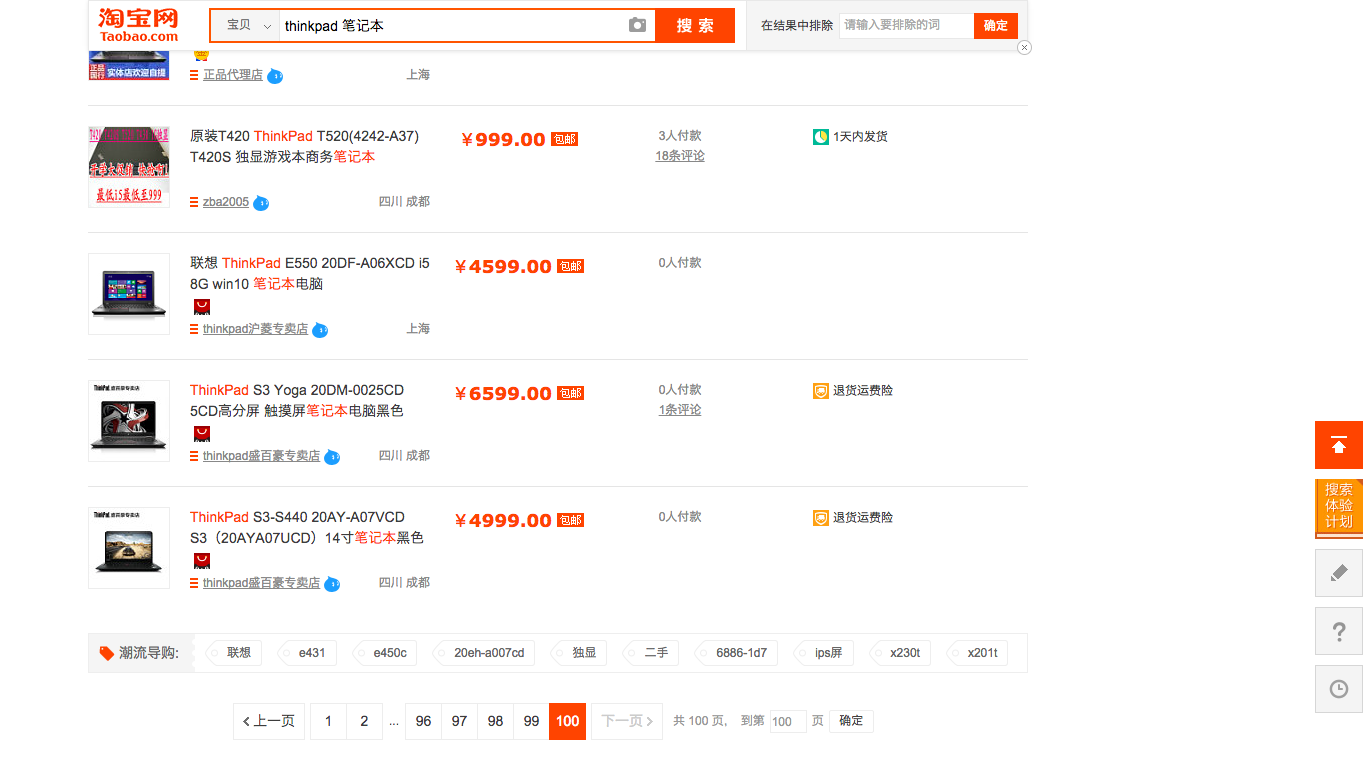
\includegraphics[width=0.9\textwidth]{hl_taobao}
		\figcaption{淘宝购物搜索图}
		\label{fig:hl_taobao}
	\end{figure}
	其实,作为互联网电子商家的翘楚---淘宝,一直在思考如何让自己平台下的优秀商品不埋没在大数据洪流中,因此,淘宝技术团队一直把个性化推荐系统视为解决用户-商品合理匹配的终极杀手锏。对于一个电商平台,原则上商品肯定是多多益善,但对于一个个性化推荐系统,则遵守更少,但更好的原则,推荐系统代表了一种自律的、精要的生活方式,据笔者所知,已经有很多互联网企业已经或者正在开发符合其企业文化的推荐系统,如笔者曾供职过的小米、今日头条和滴滴出行,其中小米的广告部门很早就利用推荐算法实现旗下各个业务线的只能广告投放,而今日头条利用推荐系统每日为用户定时推荐文章,滴滴出行则利用推荐系统为每个乘客和网约车做定向匹配。对于传统的推荐系统,首先,需要积累足够多的商品信息,因为只有尽可能的在基于所有的商品大局观上,才有可能得出比较正确的商品推荐候选集合;其次,需要尽可能积累用户的行为数据,因为这些数据将会是推荐统计假设检验的唯一数据标准,统计学之所以常让人意外,就是因为人们常常只能得到一部分的样本,而这些样本只是包含了部分而不是全部数据的信息,就有扭曲事情本质的趋势,因此,精度是推荐系统最重要的指标之一,后文会详细介绍如果通过用户画像和用户兴趣\citep{user-interests-explore,user-interests-explore1,user-interests-explore2,user-interests-explore3,user-interests-explore4}提升推荐系统的精度;最后就是甄别,哪些商品对哪些用户有着非同寻常的吸引力,其实对于一个用户来讲,平台上存在的绝大多数商品,包括数据、资源和他人观点,都没有什么价值,只有少数商品效果非凡,影响巨大,推荐系统的核心就是算法,通过算法甄别无意义的多数,只留下有意义的少数。总之,通过算法分析用户兴趣,分析商品特性,为每一个人,对所有商品打分、排序、取topN,找到用户感兴趣的商品,然后得出推荐结果,给用户他们想要的。

	但是,传统的推荐系统也有一些问题,典型的有数据稀疏问题、新用户问题、马太效应、实时推荐问题和用户兴趣变动问题。数据稀疏问题的本质就是商品信息数据过于膨胀,即使是骨灰级用户也没办法穷尽百分之一的商品,因此大多数的用户-商品相关值都是零,这不利于推荐系统做出正确的推荐结果;新用户问题又叫冷启动问题,指一个用户刚刚注册登录,推荐系统没有与此人相关的信息,于是就没有方法做出推荐;马太效应是指越热门的商品越有被推荐的趋势,这种情况其实不是一件好事,因为:1,商品营收不平衡会增加平台的风险性,如果平台大多数营收的贡献来自于若干类商品,一旦这类商品发生问题,平台也会有问题;2,根据2/8原则,冷门商品虽然营收少,但它们的基数大,潜力无限;实时推荐问题是指用户从浏览到购买这段时间一般很短,而推荐系统需要打时间差,在用户购买之前就做出推荐,但这是很难实现的,因为对所有商品打分、排序、取 topN,最后找到用户感兴趣的商品,在工程上是需要一些时间的;用户兴趣变动问题是指用户兴趣是一个动态的过程,有可能随着季节周期性变动,有可能随着年龄发散性变化,推荐系统需要及时收集数据,保持对用户兴趣的最优拟合。

	基于这些问题的存在,笔者基于推荐系统实现了用户画像模块和用户兴趣探索模块,帮助推荐系统做出更好的推荐结果。用户画像模块其实就是回归了问题的本质:以人为本,用数据说话。通过分析、收集所有与用户有关的数据,为每个用户建立、维护一个独一无二的用户画像,用户画像的最大优点在于它能主动收集用户的基本人口数据、长期兴趣和短期兴趣,而且用户画像中的信息是动态更新的,也就是说随着时间的推移,用户的兴趣在逐渐改变,用户画像里的兴趣标签也会随之改变,最大程度上保证了用户兴趣的连续性和变化性;用户兴趣探索模块包括三个原则:1,用户和潜在感兴趣商品的关联度很低,这保证了探索的商品都是用户从前没有看见过的;2,用户满意度很高,这是通过利用用户行为,包括点击次数、滑屏次数、滑屏频率、滑屏时长、点赞、分享等行为,量化了用户的满意度;3,潜在商品的标签是小众的、冷门的标签,因为热门商品是没必要也不需要做探索的。

\section{推荐系统的简介}
推荐系统的研究其实是个交叉学科,因为其跟很多早期的基础领域的研究相关,比如认知科学\citep{cognitive-science},信息检索和预测理论\citep{Forecast-principle}。随着数据时代的到来,研究人员开始研究如何利用用户对商品的行为数据来预测用户的兴趣,同时为用户提供推荐服务\citep{cf-sn}。近些年来,推荐系统越来越开始成为一个专门的研究课题,到2005年左右为止推荐系统的研究还是集中在基于user、item的协同过滤算法\citep{Wikipedia},在工业界目前应用最具有影响力的算法应该就是亚马逊的协同过滤算法\citep{Amazon-cf}。推荐系统推荐有俩个原则:1,给用户的商品不能与用户购买过的商品重复;2,不能与用户刚浏览过的商品太相关。推荐系统的函数形式化定义:设C是所有用户的集合,S是所有可以推荐给用户的主题的集合。实际上,C和S集合的规模通常很大,如亿级别的顾客以及百万级别的商品。设函数u()可以计算主题s对用户c的推荐度R,即$u=C\times S \rightarrow R$,R是一定范围内的全序的非负实数,推荐要研究的问题就是找到推荐度R最大的那些主题S*,如\autoref{equ:fromal}。
\begin{equation}
\forall c \in C,S^{*}=arg  max_{s \in S} u(c,s)
\label{equ:fromal}
\end{equation}

	\subsection{推荐系统的产生与发展}
	随着计算机存储技术以摩尔定律指数增长,信息的传播也开始爆发式的迅猛发展起来,我们这个时代的人类社会进入了一个崭新的大数据信息时代:互联网和物联网几乎无处不在,影响人类的衣食住行等方方面面,因此颠覆性的更改了人们的生活方式,在典型的互联网共享经济平台,一个用户既代表了消费者,也代表了生产者,就如笔者在滴滴出行的角色,平时上下班打车,属于运力消费者,周末开车做网约车司机,则变身为运力生产者。但是不好的一面是,曾几何时笔者发现自己社交账号开始多起来,数量之多以至于没办法记住每个账号的密码。这就是Web 2.0时代的一个副作用---让人们疲于奔命的把生活浪费在刷各种动态、信息,忙于各种无脑点赞、分享,而没有时间思考。社交化网络媒体如微信、微博的异军突起,导致互联网中的信息数据中充满了广告和噪声,而非IT行业的用户一般缺少过滤、屏蔽噪声的主观意愿和技术能力,不仅使其信息检索的时间成本巨大,也会让其在茫茫多的数据海洋里迷失自我,这就是信息过载问题的根源所在\citep{info-overload, info-overload:1}。作为非常重要的技术手段,推荐系统和搜索引擎为用户解决信息过载提供了不可或缺的保障。倆者的不同之处在于:搜索引擎是分散的、被动的,用户需要先输入关键词,搜索引擎根据关键字在服务器后台进行信息检索,利用算法获得最优的匹配信息并展示给用户。但我们更多时候遇到的问题是,并不能精确描述自己的需求,而这就是推荐系统的强项,因为推荐系统是主动收集用户平日中一点一滴的数据,以至于用户不需要提供明确的需求,推荐系统只是通过分析用户的历史行为数据就可以“猜出”用户的意图,因此,如果我们把推荐系统和搜索引擎看作为两个互补的技术手段,那么效果一定很棒。

	推荐系统最开始的概念,应该是在1995年由美国人工智能协会\citep{recmd-history}上的Robert Armstrong教授首先提出,不仅如此,其实现并不遗余力的推广了一个推荐系统的原型系统。受其启发,推荐系统的研究工作开始起步并发展壮大。第一个商用推荐系统应该属于Yahoo网站的个性化入口MyYahoo。到了21新世纪,随着电子商务的风起云涌,推荐系统的研究与应用开始水涨船高,包括eBay、taobao、Amazon、youtube\citep{recmd-youtube}等各大电子商务网站都有了自己的推荐系统,其中,Amazon公司称其网站中百分之三十的营业额的流量入口来自于推荐系统。2006年美国的Netflix\citep{recmd-netflix}在网上公开了一个推荐算法竞赛,设立了丰厚的奖金,选手通过利用Netflix公开了的真实网站中的一部分数据,包含用户对电影的评分,利用数据挖掘算法预测哪些用户会购买哪些电影。2014年阿里举办了阿里大数据竞赛,笔者和小伙伴有幸参加并顺利进入决赛,阿里公开了其部分用户三个月的浏览、收藏、购买商品数据,选手可以利用阿里天池计算资源做出预测,阿里大数据竞赛有效地推动了学术界和产业界对推荐算法的兴趣,很多有效的算法在此阶段被提了出来。

	随着互联网企业深入人心的发展、壮大,推荐系统在电子商务中的优势地位也越来越明显。国内比较典型的电子商务平台网站有淘宝网、网易云音乐、爱奇艺PPS等。在这些电子商务平台中,网站提供的商品数量不计其数,网站中的用户规模也是亿级别的。据双十一官方统计,天猫商城中的商品数量已经超过了5000万。试想下,在如此庞大商品数量的电商网站中,如果用户仅仅依靠搜索引擎输入关键字查询,过滤掉百分之九十九的商品,剩下百分之一的商品还是有太多的相似结果,只会让用户更难区分。淘宝网在这一块做的很好,其手机app主页的推荐系统能够根据用户浏览行为\citep{user-interest}及时的为用户推荐商品,笔者发现淘宝的推荐结果已经成为大部分用户的主要购买入口,总的来说,目前比较成功的电子商务网站中,都在利用推荐系统这只会下金鸡蛋的母鸡,在用户购物的同时为用户推荐一些商品,从而提高商品的销售额。另一方面,随着以iOS、Android系统为代表的物联网引领了移动互联网的发展潮流。在用户在接入移动互联网过程中,其经纬度信息可以被非常准确地被获取,因此出现了大量的基于用户位置信息推荐系统。国外比较著名的有Uber和Coupons。国内著名的有滴滴出行和美团网。美团网这种基于互联网的外卖平台,会利用位置服务为用户可推荐当前位置的餐馆、酒店、影院、旅游景点。线上交易,线下消费,之后为自己在现实世界中的体验打分,分享自己的经验与感受,形成线上下单-线下消费-线上评价的生态闭环。只是当笔者使用美团基于位置的美食服务时,同样也会遭遇信息过载问题,矛盾在于商家太多了,而笔者只能一次去一家餐厅就餐,这时美团平台的推荐系统会根据笔者的历史消费信息,加上笔者的偏好、口味、消费能力等,为笔者推荐当前位置下最可能感兴趣的餐厅。

	随着网络社交的深入人心,用户不再满足于单纯的获取信息,而是与网络上的其他用户进行关注、聊天和互动。国外著名的社交网络就有Twitter、Facebook等,国内的社交网络有微信、微博等。在社交网站中用户不再是一个静止端点,而是与他人有错综复杂关系的社交网络。对于微信来说,最重要的资源应该就是用户之间的关联。这其中的关系可能是多层次的、多维度的、按时间序列走的,关联的因素可能是是亲人、好友、同学、同事,也可能只是网络中的萍水之交,如都是QQ黄金会员。因此,用户之间的关联应该有一个权重,表明了用户之间的紧密度、信任度,一个用户的联系人A可能是其好友A的亲戚,而A可能对这位亲戚的存在一无所知,因此推荐系统有助于帮助用户挖掘潜在的熟人。

	由此可见,推荐系统在很多领域取得了她们应有的地位:滴滴出行的网约车推荐、淘宝平台的商品推荐、美团的美餐推荐、电影推荐和音乐推荐,囊括了人类的吃住行穿四大领域,团购网站美团网早已经利用推荐系统提供面向不同业务的个性化服务:1,猜你喜欢:美团最重要的推荐产品,目标是让用户打开美团App的时候,可以最快找到用户想要的团购服务;2,首页频道推荐:若干频道是固定的,若干频道是根据用户的个人偏好推荐出来的;3,今日推荐个性化推送:美团的个性化推送的产品,目的是在用户打开美团App前,就把用户最感兴趣的服务推送给用户,促使用户点击及下单,从而提高用户的活跃度;4,品类列表的个性化排序:美团首页的那些品类频道区。

	自诞生后,学术界对推荐系统的关注度一直不小。从1999年开始,在美国每年由计算机学会负责召开电子商务研讨会,会中已经发表了数以千计的推荐系统论文。在2001年,ACM信息检索专业组考虑把推荐系统独立拆分,作为会议诸多独立研究主题之一。2001年同年,在人工智能联合大会上,推荐系统也单独列为一个主题。2011年的KDD CUP 竞赛中,两个竞赛题目分别为音乐评分预测和识别音乐是否被用户评分(\href{http://www.kdd.org/kdd2011/kddcup.shtml}{www.kddcup2011.org})。2012年的KDD CUP 竞赛中,两个竞赛题目分别为腾讯微博中的好友推荐和计算广告中的点击率预测。(\href{www.kddcup2012.org}{www.kddcup2012.org})

	\subsection{推荐系统的应用}
	作为IT数据挖掘算法工程师,笔者经常听到同事开玩笑的说:推荐系统就像万金油,抹哪哪灵。对于诸如linkedin的社交网络,推荐系统改变用户扩展人脉的模式和方法,而这是基于一种假设:你的朋友的朋友有可能就是你熟悉的人。对于诸如淘宝的电商平台,搜索提供的静态体验,并不足以让用户产生购买欲望,推荐系统加强了交互,包括用户和商品、用户和用户,一个人的消费可能带动一群人模仿,成就了一种极致的营销模式。对于诸如滴滴出行的网约车平台,给定某一时刻、起始经纬度、终点经纬度、车型,根据推荐算法一定会有一个最优派单,使得司机和乘客所得的好处,远远大于平台的抽成费用,形成了我们所说的三方共赢,只有倒霉的传统出租车利益受损的局面。总体说来,一个成功的个性化推荐系统的作用主要表现在以下几个方面:
	\begin{enumerate}[(1)]
	\item 将潜在用户转变为购买者:用户在浏览的同时并不意味着一定是要消费,也许只是看看,遇到合适就买,没有就算。个性化推荐系统的职责之一是能够洞察用户的潜意识,帮助用户找到其感兴趣的商品,从而促成购买过程。
	\item 提高平台的连带销售能力:有时候个性化推荐系统需要一点联想能力,如用户购买了手机,那么推荐手机壳就是一种明智的联想,会让用户产生“你懂我”的感觉。
	\item 提高客户对平台忠诚度:个性化推荐系统就是那个时时刻刻为用户着想的机器人,每一次推荐只是那么一点点,不是很多,但都很好,这种依赖就是俞军先生所说的体验壁垒,对于用户来讲,从滴滴出行换到Uber,功能还是原来的功能,只是用户习惯的打车方式都变了,以至于无法接受Uber。
	\end{enumerate}

\section{用户画像的简介}
	用户,指企业的潜在消费者,是构成现有用户的大部分群体的统称。画像,是对一个用户的可视化、客观的描述。用户画像就是能够客观、可视化地描述潜在消费者的模型。用户画像建模的关键工作就是为用户打上合适的标签,标签通常是人为规定,且具有高度精炼的特征标识,如消费能力、偏好、年龄、性别等,将所有用户标签综合起来,抽象出本质,如忠诚度、消费度、满意度等,基本就可以勾勒出该用户的部分轮廓。
	\subsection{用户画像的产生背景}
	当互联网步入信息时代后,用户行为数据的极大丰富性给企业及消费者的消费行为带来一系列问题与变革。最大的问题在于电子商务的用户数量相比传统商务,膨胀了成百上千个数量级,单纯依靠人工方式已对其无解,2015上半年,我国网民已达到6.68亿,预计年底能够顺利突破7亿,其中使用手机上网人群占整体88.9\%,而手机上网存在着独特性、唯一性和私密性的特点,每个人的手机都是一套独特的生态系统。最大的变革莫过于,消费者的一切行为信息都是可数字化,随着大数据工程技术的日益精湛,带宽、计算资源、存储资源也变得极大丰富起来。这使得企业有能力把专注点回归到问题的本质,即利用信息化管理方式为每位用户建立一个档案,根据用户的生活习惯、消费行为和社会属性等信息,抽象出的一个标签化的用户模型用以精准刻画用户,基于此进而充分挖掘用户潜在的商业价值,随着用户使用时间越长,模型就越能积累多的数据,也越能精确把握用户的消费习性,反过来越能促使用户的消费行为,形成一个良性循环,至此用户画像的概念也就深入企业和用户之心。

	大数据时代的用户行为数据就像是做饭的米,如果想让其变成香喷喷的白米饭,还面临很多问题:1、用户行为数据通常包含了很多的噪声,包括用户无目的地的浏览数据、用于营销目的的分享数据、用于作弊的刷单数据等等,这些数据并不能够代表用户的真实意图甚至有时代表的是相反的意愿;2、用户行为数据通常需要将其所包含的意义抽象化,才有利用价值,比如根据用户最近一个月的浏览、购买记录,通过分析、抽象、挖掘得出用户的活跃度、消费能力和忠诚度,这才能为算法所用;3、用户行为是是一个不断迭代的行为,如何均衡新旧行为数据的权重比,是一个很严肃的问题,比如一个用户上一个月购买不断,最近一个月却很少登录,那么我们应该怎么归因用户的这种行为?以及如何刻画这个时期的用户消费状态?如果用户处于将要流失的状态,又该如何做;4、不管到哪,我们总会遇到与自己志同道合的其他用户,我们其实还是比较关心这些人的选择,如果能拿来做为自己的参考也不是一件坏事,因此,如果存在一种机制,可以将有相同特征的用户抽象成一个代表,一视同仁,则既方便用户消费又能促进企业营收。基于以上种种问题,我们确定选用了用户画像。
	\subsection{用户画像的应用}
	用户画像建模的过程,就是数据清洗、数据分析、数据挖掘,最后得出用户的抽象概念的过程,用户画像的本质就是了解企业的用户,然后完善产品运营提升用户体验,提升盈利,用户画像可以为包括推荐系统、运营推广、策略制定等提供数据支持。除此之外,用户画像可以帮助企业寻找潜在目标用户,在与用户的交互上了解其偏好,促成购买,实现精准运营和营销,用户画像改变了以往闭门造车式的商业交易模式,通过事先调研用户需求反馈,设计制造出更适合用户的产品。具体来讲,用户画像的应用包括:
	\begin{itemize}
	\item 完善及扩充用户信息:用户画像代表了用户的信息全貌,因此寻找足够多的数据是用户画像建模的前提条件。我国在各方面都是很大的长尾市场,互联网很大程度上弥补了信息的不对称,移动互联网又让把信息在精准送达到任意一个用户面前,尽管如此,根据2/8原则还是导致了大多数的用户和商品的数据是空缺着的。同时,在实际中用户的信息也可能提供得不尽完整,如对于没有填写性别信息的用户,用户画像可以通过用户兴趣探索模块,生成用户数据,可见,用户画像不仅消费数据,也可以生成数据。
	\item 打造健康的生态圈:在掌握用户信息的基础上,电子商务平台就可以对自身的状况进行分析,从相对宏观的角度刻画用户种群的分布,从基础上把握市场的生态环境,挖掘出商品的最大价值,帮助企业提高收入。例如笔者曾经发现,通过与当前热门电影保持同步,通过适时发布引导疯传引爆点、跟进推广周边手机主题,可以很好的带动用户的消费行为,用户的消费与此同时也刺激了第三方设计师紧跟时尚潮流,尽可能第一时间发布引领流行的作品。
	\item 支撑推荐系统的精准推荐:精准推荐的前提是对用户的清晰认知。在实际场景中,影响用户对商品的使用黏度的因素很多,在这种情况下,利用用户画像可以对用户的“贴身跟踪”就能及时发现薄弱环节,因此从用户打开应用网上商店到退出使用,其间的每一步情况都被快的记录在案:哪一天退出的,哪一步退出的,退出之后“跳转”到什么软件等等。据此,用户画像也实现了用户另外一个纬度的归类,分清哪部分是忠实用户,哪部分可能是潜在的忠实用户,哪些则是已经流失的;更进一步来看流失的原因:因为代金券没有了流失?主题包质量不好流失?这些都是下一步精准推荐的依据,无论是基于兴趣的推荐提升用户价值,精准的广告投放提升商业价值,还是针对特定用户群体的内容运营,用户画像都是其必不可少的基础支撑。直接地,用户画像可以用于兴趣匹配、关系匹配的推荐和投放;间接地,可以基于用户画像中相似的兴趣、关系及行为模式去推动用户兴趣和设计师的无缝对接。
	\item 市场安全领域的应用:有时候商家会通过各种活动形式的补贴来获取用户、培养用户的消费习惯,但同时也催生一些通过刷排行榜、刷红包的用户,这些行为距离欺诈只有一步之遥,但他们的存在严重破环了市场的稳定,侵占了活动的资源。其中一个有效的解决方案就是利用用户画像沉淀方法设置促销活动门槛,即通过记录用户的注册时间、历史登陆次数、常用IP地址等,最大程度上隔离掉僵尸账号,保证市场的稳定发展。
	\end{itemize}

\section{工程背景}
	小米科技有限公司作为国内发展较快的互联网企业,活跃用户过亿,移动端用户比例高,有着大量的用户和丰富的用户行为,这些为推荐系统的应用和优化提供了不可或缺的条件,我们基于MIUI主题应用商店开发的手机主题推荐系统,作为用户和主题包之间的桥梁,体现出超强的变现能力。但现有的手机主题推荐系统也面临着一些问题。
	\begin{enumerate}[(1)]
	\item 新用户冷启动问题。当前使用的推荐算法,包括最近邻的协同过滤算法、PageRank排序算法、关联规则挖掘是根据给定用户对某些物品的行为数据,给每个用户推荐Top-N个其最喜欢的物品,当一个新用户进入一个站点时,我们对他的兴趣爱好还一无所知,这时如何做出推荐是一个很重要的问题。现有的机制是向用户推荐那写普遍反映比较好的物品,也就是说,推荐完全是基于物品的,这就会使热门的商品越来越热,冷门的商品越来越冷,代价就是加剧了热门商品的马太效应。

	\item 数据稀疏问题,通过观察我们发现只有约20\%的用户有过多于5款主题行为记录,意味着大多数主题包处于待挖掘状态,然后,这又是一个蛋和鸡的问题:要形成好的推荐,首先需要有大量的用户行为支持,这样才能得到足够多的推荐数据,这里问题的关键在于推荐系统如何首先能在数据稀疏的情况下给出优质的服务,打破这个闭环。

	\item 不断变化的用户喜好,这个问题主要分为俩类:1、用户一直喜欢某种类型的主题包,只是长时间没有机会接触,如一位男性用户喜欢美少女主题包款式,虽然不会主动查找,但如果不经意看到一款制作精美的美女主题包,可能还是会购买,这就是用户的长期兴趣。2、用户之前喜欢某种类型的主题包,之后转为喜欢另外一类主题包,如用户刚开始喜欢清纯系,后来转为温柔系,这时如果向用户推荐温柔系主题包更有可能被其接受,这就是用户的短期兴趣。

	\item 重复推荐的问题,手机主题包属于电子虚拟商品,它的特性是第一次下载需要购买,之后下载则免费,现有的推荐系统会重复推荐用户之前购买过的主题,导致占用有限的推荐位来显示无法变现的信息,并且会给用户一种不专业、不智能的体验。

	\item 其他问题,如推荐商品长尾性有待加强、隐性喜好\citep{latent-cf}难以挖掘、偏激的用户和另类的产品、推荐系统的作弊行为、用户请求量大等。这些问题相对来讲影响范围小,本论文不做过多讨论。
	\end{enumerate}

	我们发现,如果在底层数据仓库层和推荐系统之间加一个用户画像模块,会有效提升推荐系统的各项性能。1、对于新用户冷启动问题、数据稀疏问题,关键是收集足够多的用户基本信息,在没有或者只有少量用户行为的情况下依靠用户画像对用户推荐比较合理的主题。2、对于不断变化的用户喜好,我们通过用户画像存储用户用户长期,通过用户兴趣探索获得用户短期兴趣,并针对手机主题市场的特点,利用线性衰减算法融合用户画像和用户兴趣探索,使得推荐结果能兼顾俩者。3、对于重复推荐的问题,我们在用户画像中维护一个白名单,用来存储用户曾购买过的所有主题信息,格式为(userId,itemId,buyTime)这样的三元组,避免向用户推荐已购买过的主题。除此之外,我们也通过探索用户小众兴趣提升推荐系统的长尾发掘能力,加强了对小众主题包的推荐力度。主要思路是分析用户所有的行为数据,针对占大多数的冷门主题(即包含小众标签的主题)会赋予一个倾斜因子,这样会使得冷门主题更有可能被探索出来。

	总之,我们采用构建用户画像的办法分析、处理、挖掘现有的用户信息,尽可能多的识别用户基础特征和兴趣偏好,达到精细化推荐的目的,后续包括定向广告投放、市场营销等功能需求都是围绕建立更细致、准确的人群画像展开。
\section{推荐系统开源项目介绍}
工欲善其事,必先利器,关于大数据,有很多令人兴奋的事情,但如何分析、利用好如此多的数据也带来了很多困惑。好在开源观念盛行的今天,有一些在大数据领域领先的免费开源技术可供利用。
\begin{itemize}
	\item Redis:Redis是一个remote类型的内存数据库,它不仅性能强劲,可扩展性好,而且还具有高效的复制特性,生来就是为解决实际问题而设计的数据模型。在实际工程中,笔者利用redis做俩件事情:1、存储计数指标,包括用户浏览、下载、购买等行为的次数,以天为单位,因为内存有限只存储最近一个月的数据;2、存储最近俩周的行为数据,按照timelines格式存储,天然支持时间排序。key有用户id,商品id,交易id,value格式为商品类型:商品价格:折扣,score为下单时间戳。
	\item Apache Hadoop:Hadoop是由大名鼎鼎的Apache基金会所开发、维护的一个分布式系统,是第一款开源的用于分布存储大型数据集的开源框架,助力各企业迅速从海量数据中挖掘出“金子”。在实际工程中,每日凌晨,把当日的MySQL DB中的数据复制一份到hdfs文件,partition为当天时间。
	\item Apache Hive:Hive是著名社交网络公司facebook开源的在Hadoop上的数据仓库基础构架。Hive的使用方式如传统的DB,类似SQL查询语言。同时,hive也帮助用户屏蔽具体的 MapReduce开发,因此十分适合大量数据的统计分析。实际工程中,笔者利用hive计算超过一个月的数据计算,其小时级别的计算时间限制了其只能适用于离线计算。
	\item Apache Spark:Spark是加州大学伯克利分校所开源的基于内存的通用并行计算框架,同时spark如hadoop一样容易扩展,因此适和完成数据挖掘需要大量计算迭代的任务。实际工程中,笔者利用spark自带的机器学习mllib库做推荐系统的模型训练。
	\item Apache Kafka:Kafka 是美国求职社交公司linkedin开发、开源的一种高吞吐量的分布式发布订阅消息系统,可以轻松处理现有所有大交易规模的用户行流数据,包括今日头条、滴滴出行级别的交易量都是利用kafka做导流。kafka的一个应用特点是实时性高、吞吐量巨大,任何要求实时处理的应用场景,Kafka都是一个可行的解决方案。实际工程中,笔者利用kafka流作为redis数据的上游数据源。整体数据流结构为:app->mysql db->mysql binlog->kafka->清洗、去重kafka->redis。从app到redis理论延迟为毫秒级别,其中的kafka是关键实现部件。
\end{itemize}

\section{论文结构}
	本文的其余正文内容由以下章节组成:
	\begin{itemize}
		\item 第二章首先介绍了推荐系统基本概念和排序模型,包括数据挖掘算法\citep{date-mining}和信息提取技术\citep{info-retrieval}的应用,然后详细介绍了用户画像和用户兴趣探索。
		\item 第三章主要讨论了如何利用用户画像建模解决推荐系统的冷启动问题,从而改善推荐系统的新用户留存率。最后给出了相关的实验结果及分析。
		\item 第四章主要讨论了如何利用用户兴趣探索跟踪用户动态并挖掘用户小众兴趣,从而提升推荐系统的长尾效应\citep{long-tail},文中给出了相关的实验结果及分析。
		\item 第五章是论文的结束语和展望,在对目前工作简要总结的基础上,提出了推荐系统下一步研究的任务和方向。
	\end{itemize}
   \chapter{基于用户画像的推荐系统综述}
	\section{引言}
	自从1992年著名的施乐公司的科学家们为了解决困扰已久的信息负载问题,第一次从概念上提出协同过滤的算法模型。1998年,林登及其同事们成功申请了item协同过滤技术的专利,经过多年的工程实践,美国电商亚马逊公司的工程师们骄傲的宣称:在公司所有的销售量,推荐系统占比已经占到整个Gross Merchandise Volume的百分之三十以上。不久之后的美国公司Netflix,因为其创始人与前任公司签署有若干年内不得从事同行工作的限制,于是通过举办推荐算法优化竞赛绕开限制,用以开发出更好的推荐算法。此次竞赛吸引了数以千计的团队参与角逐,期间进行了上百种的算法模型组合、优化的尝试,虽然Netflix公司为冠军团队支付了百万美金,但回报是Netflix推荐系统的快速发展以及营收的俩位数增长。其中冠军团队凭借Sigular Value Decomposition和Gavin Potter跨界引入的心理学方法进行的组合算法模型,在诸多优秀团队中脱颖而出。其中,矩阵分解的核心是将一个非常稀疏的用户评分矩阵R分解为两个更小的矩阵:只包含User特性的矩阵P和只包含Item特性的矩阵Q,利用P和Q相乘的结果R'来拟合原来的评分矩阵R,使得矩阵R'在R相同位置之间的损失函数值尽量的小,通过定义一个R和R'之间的距离计算公式(一般为曼哈顿距离),如果矩阵R'是正定矩阵,那么把矩阵分解转化成梯度下降求解的局部最优解,就是全局最优解。与此同时,Pandora、LinkedIn、Hulu等网站在个性化推荐领域都展开你争我抢的竞争势头,使得推荐系统在各个细分行业、垂直领域开始全面开花,都有了不少爆发性进展。但是,对于拥有全品类的综合性购物电商、广告营销,推荐系统的进展还是缓慢,主要原因是因为不同类型的商品,消费者的心态也是不同的,例如大型家电,消费者肯定是先看了又看、选了又选,从价格、定位、功能到噪声比、性价比,大多数都会先做足了调查,才会购买;与此相反,对于日常用品消费者可能眼睛都不眨就购买了,对于这俩种极端的消费情况,推荐系统需要做出截然不同的推荐策略,具体的,单个模型在母婴品类的推荐效果还比较好,但在其他品类就可能很差,很多时候需要根据场景、推荐栏位、品类等不同,设计不同的推荐模型。同时由于用户兴趣随时间会不停的变动\citep{user-interests-explore,user-interests-explore1,user-interests-explore3,user-interests-explore4},需要一种机制,使得推荐系统能定期对数据进行评估、分析,除此之外不同类型的商品有不同的更新频率,这就对推荐系统提出了更加智能化的挑战。还有,如果定期更新模型,则可能会因为计算资源的限制损害推荐的实时性\citep{temporal-cf},因为模型训练需要一定的cpu计算时间,而传统的Hadoop的方法实在是无法进行大的更新频率,spark框架又因为昂贵的内存限制了其应用场景。

	传统推荐算法包括基于人口统计学的推荐\citep{social-filter}、基于商品内容的推荐\citep{content-based}和user-based/item-based的协同过滤\citep{collab-filter}的推荐等都有冷启动问题。基于内容的推荐对物品冷启动问题免疫,但是无法解决用户冷启动问题\citep{cold-start}。

	由此,笔者在实际工程中,针对传统推荐算法的种种弊端,选择了用户画像。伟大的数学家、计算机学家Knuth先生说:如果遇到一个不好搞定的问题,那么就该添加一层中间层,用以屏蔽掉问题。实际上,用户画像作为底层数据仓库和上层推荐系统的缓冲层,起的就是这种作用。

	\section{用户画像的研究现状}
		\subsection{用户画像的组成部分}
		基于内容和用户画像的个性化推荐,有两个实体:内容和用户。需要有一种文本机制联系这两者的东西,我们定义其为标签。内容特征文本化为标签即为内容特征化,用户兴趣文本化标签则称为用户特征化\citep{user-profile,user-profile1,user-profile2,user-profile3,user-profile4}。因此,对于基于用户画像的推荐,主要分为以下几个关键部分:
		\begin{enumerate}[(1)]
		\item 标签库

		标签是联系用户与用户、用户与商品、商品与商品之间的纽带,也是反应用户兴趣的重要数据源,标签的最终用途在于标记用户行为。标签库则是对标签进行聚合的系统,包括对标签的管理、更新等。在用户画像的过程中有一个很重要的概念叫做颗粒度,就是我们的用户画像应该细化到哪种程度。举一个极端的例子,如果“用户画像”最细的颗粒度应该是细到每一个用户每一具体的生活场景中,但是这基本上是一个不可能完成的任务,同时如果用户画像的颗粒度太大,又会影响推荐精度,一般来说,标签是以层级的形式组织的,如体育为一级维度、篮球为二级维度、NBA篮球为三级维度等。

		\item 内容特征化

		内容特征化即给商品打标签。目前有两种方式:人工打标签和机器自动打标签。在实际工程中,主题推荐系统采用人工打标签方式,具体就是提供一个关键字库,供设计师从中选择适当关键字作为作品的标签。

		\item 用户特征化

		用户特征化即为用户打文本标签。通过用户的行为日志和一定的模型算法得到用户的每个标签的权重。用户对内容的行为:点赞、不感兴趣、点击、浏览。对用户的反馈行为如点赞赋予权值1,默认为0,不感兴趣为-1;对于用户的浏览行为,则可使用点击、浏览作为权值。对商品发生的行为可以认为对此商品所有标签的行为。用户的兴趣是时间衰减的,即离当前时间越远的兴趣比重越低。时间衰减函数使用1/[log(t)+1], t为事件发生的时间距离当前时间的大小。要考虑到热门商品会干预用户的标签,需要对其标签进行降权。
		\end{enumerate}

		\subsection{用户画像的构建周期}
		用户画像,即用户信息标签化,就是企业通过收集与分析消费者社会属性、生活习惯、消费行为等主要信息的数据之后,获得用户的数据标签库。构建周期如\autoref{pic:userprofile_process}。
		\begin{figure}
	    \centering
	      \framebox{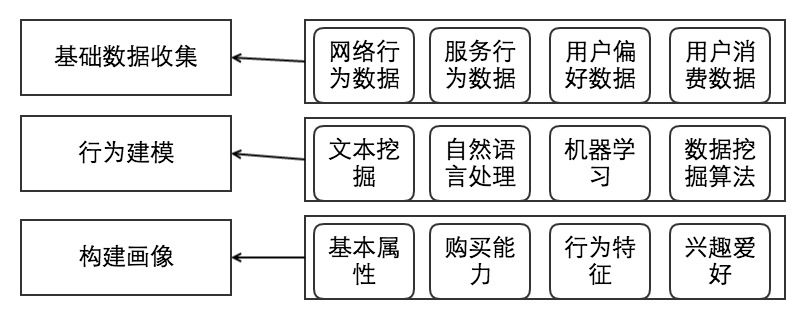
\includegraphics[scale=0.45]{figures/userprofile_process}}
	      \figcaption{用户画像的构建周期示意图}
	      \label{pic:userprofile_process}
	    \end{figure}
	    \begin{enumerate}[(1)]
	    \item 数据收集

	    数据收集大致分为四类:1、网络行为数据包括页面浏览量、活跃人数、访问时长、浏览注册转化率、注册活跃转换率等。服务内行为数据:点击浏览路径、网页停留时长、滑屏次数、滑屏频率、滑屏时长。用户内容偏好数据:点击、浏览、收藏内容、评价、评分、评论内容、社交内容、品牌偏好等。用户交易数据(交易类服务):购买率、折扣率、导流率、流失率等。收集到的数据没必要是百分之百的准确,大体差不多即可。应用中,具体就是在数据清洗阶段过滤一部分不靠谱的异常值,验证、更新数据这块需要在后面的阶段再做判断,比如某用户在性别一栏填的女,但其语言数据显示其为男的概率更大,根据业务再选择丢弃数据还是更新数据。
	    
	    \item 行为建模

	    该阶段是对收集到数据进行建模,目标是抽象出用户的文本标签,这个阶段不应该再纠结数据的正确性,而是应该注重大概率事件,通过统计学假设检验尽可能地排除用户的偶然行为。这时也要用到数据挖掘算法模型,对用户的行为进行回归预测,比如已有一个线性回归函数:y=kx+b,X 代表用户行为,y是函数拟合的用户喜好度,y'是用户真实偏好,我们通过不断的训练数据,利用参数k和参数b来得出最新损失函数下的值,用以精确模拟y'。

	    \item 用户画像基本成型

	    该阶段是行为建模的深化,需要利用用户的基本属性,如性别、地域、年龄,得出用户更高层的抽象概念:消费能力、忠诚度、活跃度、社交爱好等。因为用户画像永远也无法百分百地拟合现实中的一个人,只能做的就是不断地去减小拟合的损失函数,因此,用户画像需要根据变化的基础数据不断修正已有的更高层的抽象概念,尽可能模拟用户的变化趋势。

	    \item 数据可视化

	    最后是数据可视化分析,这部分是最能体现推荐系统的产出,因为人类对数据不如对图画来的敏感,在此步骤中一般是针对群体做进一步的抽象,按照消费习惯、消费能力、消费偏好把用户归类为一类人,比如可以根据用户对价格的敏感度细分出高价值用户、核心用户、高忠诚用户。而决策层所做出的评估也应该是基于某一群体的分布规律。典型的用户画像如\autoref{pic:user_profile}。
	    \end{enumerate}
		\begin{figure}
	    \centering
	      \framebox{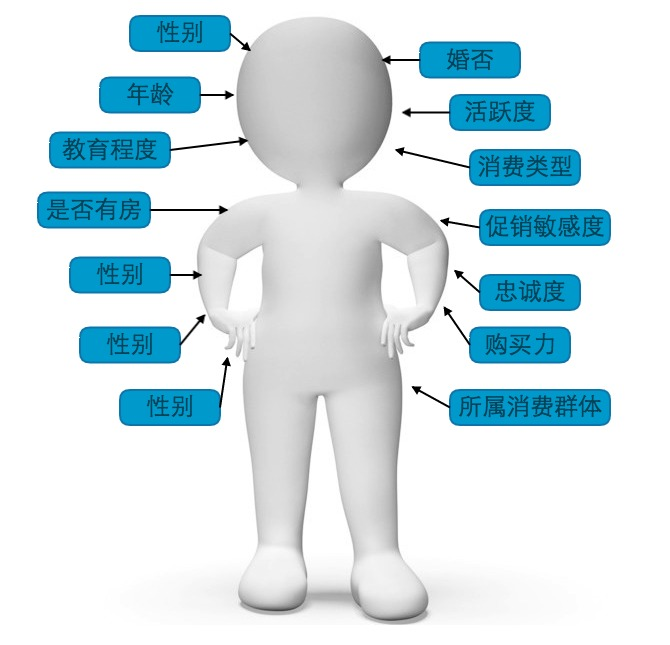
\includegraphics[scale=0.4]{figures/user_profile}}
	      \figcaption{用户画像示意图}
	      \label{pic:user_profile}
	    \end{figure}

		\subsection{用户画像的建模}
		用户画像的建模包括内容标签化和标签权重量化。建模过程:1、内容分析,从原先的物品描述信息中提取有用的信息用一种规范化的标签表示,有时候这种信息源自于作者提供的描述,有时候源自于用户的评价,不管如何,都需要人工做进一步的审核;2、上传、记录用户注册信息,生成用户基本信息,这些信息基本是不会变化的;上传、记录用户行为数据,这些数据是不断变化着的,通常是采用数据挖掘算法从潜在物品集合中取出若干个结果表示用户喜好的模型。例如,一个网页推荐系统,可以通过分析用户过往浏览过的文章,得出用户喜欢浏览类似于范冰冰的花边新闻,如果用户点击了所推荐的文章,则说明分析正确,否则需要根据反馈重新训练模型,从而实现一个反馈-推荐-反馈的闭环;3、推荐系统得出推荐集合后往往需要取topN,因为推荐系统的本质在精不在多。通过定义一个距离算法,匹配用户标签和商品标签的相关度,相关度一般正则为0-1之间,结果是一个二元的离散量:(pid, score)。根据相关度将生成一个用户潜在感兴趣的物品评分列表,然后去掉用户之前看过的商品,取topN即可。例如在电影用户画像的建模中,首先分析用户打分比较高的电影的共同特性,包括导演、演员、风格等,这些电影的标签就会成为此用户画像的一部分,根据打分的多少,给定一个合适的权重值。用户-标签用矩阵A表示,电影-标签用矩阵B表示,A乘B得出矩阵C,C代表了用户与电影之间的相关度,固定一个用户,对所有相关度不为零的电影做排序,取topN即是推荐结果。用户画像建模的根本在于用户标签的获取和权重的定量分析。

		对于商品描述,也可以做进一步的处理,丰富商品的标签集合。其实和文本处理类似,笔者选择使用目前应用最广泛的方法:TF-IDF方法。设有N个文本文件,关键词$k_{i}$在$n_{i}$个文件中出现,设$f_{ij}$为关键词$k_i$在文件$d_j$中出现的次数,那么$k_i$在$d_j$中的词频TF$_{ij}$定义为:TF$_{ij}$=$f_{ij}$/max$_zf_{zj}$,其中分母中的最大值是通过计算这个文本j中所有关键词出现的频率得出。附图给出了3个短文和5个关键词,以关键词人为例,该关键词在文本1中出现了1次,而文本1中出现次数最多的关键词是事,一共出现了2次,因此TF$_{11}$=0.5。一个关键词经常在许多文件中出现,则该关键词能表示文件的特性的意义就会较小,试想我们考察关键词i出现次数的逆,也就是$IDF_{i}$=log(N/$n_{i}$),这个想法和Adamic-Adar指数思路基本相似,关键词i在文本文件j中的权重于是可以表示为$w_{ij}$=$TF_{ij}$*$IDF_{i}$,而文件j可以用一个向量$d_{j}$=($w1_{j}$,$w2_{j}$,…,$wk_{j}$),其中k是整个文本库中关键词的个数。一般而言,向量应该是一个稀疏向量,即其中很多元素都为0。如果把用户今日点击、浏览、购买的商品抽象成一个标签向量,则可以通过用户标签向量-商品标签向量的点乘得出一个数值,从所有数值中把相似性最大的那个产品的标签更新给该用户画像,第二大相似性的产品标签权重减半更新给该用户画像,以此类推,完成用户画像的建模过程。
		\begin{lstlisting}
		文本1:不做软事,不说硬话,对事不对人。
		文本2:多少事,从来急;天地转,光阴迫。一万年太久,只争朝夕。
		文本3:青春之所以幸福,就因为它有前途。

		关键字包括人、事、硬话、一万年、朝夕、青春、幸福、前途
		\end{lstlisting}

		\subsection{用户画像和推荐系统的评测}
		首先,用户画像作为一个工具,只用在运用到某一场景才有意义,并能评估出其产出,因此本节主要介绍推荐系统的评测,根据推荐系统的表现好坏才能评估出用户画像的推荐质量。实际工程中,笔者利用A/B实验对若干组模型进行定量对比。标准的A/B实验是指通过一定的规则把类似的用户群随机分成俩组,采用旧模型的分组叫对照组,采用新模型的分组叫实验组\citep{ab-test}。通过对用户展示不同的模型,得出用户的使用指标,关键是各种转化率,这样仅仅通过对比倆者的转化率即可得出各个模型的优劣。策略实验的难点在于如何找到合适的实验设计方案。通过时间交错能够在一定程度上减少由时间片带来的误差,这样就有一个难题:  如何选择合适长度的时间片。策略实验往往伴随着携带效应(carry-over effects),也就是上一个时间片的策略会对下一个时间片带来影响。笔者和同事们提出一个方案,当选择适当大的时间片的时候,通过A/A实验的数据调整A/B实验的结果,具体来说,如果A/A实验的结果是 0.4\%, A/B实验的结果是 1.2\%。那么我们认为A/A实验是真实的时间片之间的差异, 我们需要用倆者之差的绝对值去调整时间片带来的影响,

	\section{用户画像在推荐系统的应用现状}
	Amazon的仓库里堆着数百万图书,Netflix的服务器中存储有数万部电影,淘宝平台上的小卖家总共拥有8亿件物品,除此之外,这三家公司都保留有数以亿计的用户行为数据。互联网电子商务开始积累了海量的用户数据,然后因为数据量过于庞大,有用信息如金矿中的金子一样很难挖掘利用,与此同时,用户发现常常需要面对过多的选择。心理学研究证实过多的选择会使人犹豫不决,导致消极等待,最终可能放弃消费的决定,这个问题严峻到可以造成肉眼可见的用户流失。近代统计学理论的发展加上最近几年的数据科学和数据挖掘工程的进步,为电子商务平台提供更有效的应对方案:推荐算法。推荐系统在帮助用户解决信息过载问题的同时,提升了企业价值。如今的企业不再局限于传统的推荐功能,通过建立完备的用户画像,推荐系统可以帮助企业更了解用户,在推广、反作弊、精细化运营等领域中发挥重要的作用。
		\subsection{基于用户画像的推荐系统的商业应用}
		\begin{figure}
	    \centering
	      \framebox{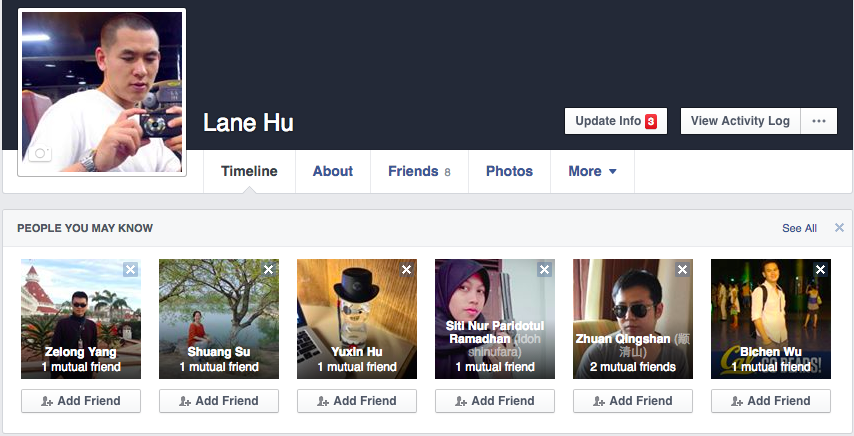
\includegraphics[scale=0.45]{figures/recmd_facebook}}
	      \figcaption{Facebook个性化推荐用户界面}
	      \label{pic:recmd_facebook}
	    \end{figure}
		作为全球社交网站中的翘楚,Facebook在很早的时候就预言到了大数据+推荐系统+用户画像的无限前景。Facebook自己的推荐系统就是需要利用分布式计算框架快速的帮助用户找到他们可能感兴趣的人、文章、分析、用户组等。Facebook是个伟大的公司,一直为开源软件贡献着一份力量,最近在其官网就公布了Facebook自己的推荐系统原理、性能及使用情况\citep{recmd-facebook}。Facebook的推荐系统需要面对的数据量应该是所有互联网公司中的数一数二,约包含了1000亿级别的评分数、10亿级别的用户数以及百万级别的虚拟商品,如何在如此庞大的数据规模下,仍然保持良好性能已经成为世界级的难题,而Facebook解决了,通过分析Facebook给出了一些实验的结果,表明,Facebook的系统比传统系统要快10倍左右。目前,该方法已经用到Facebook的多个app应用中,包括用户、用户组的推荐。Facebook推荐主页如\autoref{pic:recmd_facebook}。
		
		Facebook的用户画像进展也十分可观,几乎是与推荐系统同步发展。2011年12月,Facebook发布了里程碑式的大数据产品——Timeline,通过开发API接口,允许用户自行编辑个人的时间轴:在什么时间、什么地点做了什么,遇到了谁,可以说在这条时间线记录这个人的全部生活故事。Timeline通过帮用户回忆自己的点点滴滴的同时,完成了用户数据捕获、存储,而一旦拥有了这些历史数据,Facebook就可以做进一步的数据分析、挖掘,这时的Facebook就如同和你从小长大的小伙伴,一个懂你的陌生人。可以说用户留下的数据越多,Facebook就越了解这个人,投放的广告就会更加精准,最终Facebook利用庞大的用户数据生态赚足了钱。

		\subsection{推荐系统的主要方法}
		推荐系统主要有俩种思路:评分预测和Top-N预测,核心的目标都是找到最适合用户的候选集合s,从候选集合里挑选目标集合是一个非常复杂的非线性优化问题,通常采用的方案是用局部最优近似非线性最优,通过定义一个的损失函数,选取Top-N	\citep{recmd-Next}。

		推荐系统的算法基于统计学、概率论、线性代数、微积分技术,找出用户最有可能喜欢的商品,应该是现代互联网电商的明星应用。目前用的比较广泛的推荐算法还属协同过滤推荐算法,其基本思想是根据与他兴趣相近的用户的选择,得出推荐商品候选集,取topN推荐给目标用户,用维度为m×n的矩阵表示所有用户对所有物品的兴趣值,这个值应该是根据用户历史行为数据得出,值越高表示这个用户越喜欢,利用特殊值0表示没有接触过。图中行向量表示某个用户对所有商品的喜爱程度,列向量表示某个商品对所有用户的吸引程度,因此单个元素$U_{ij}$表示用户i对物品j的喜欢程度。协同过滤分为两个阶段:预测阶段和推荐阶段。预测阶段是基于所有原始集商品,预测这个用户有没有可能对其感兴趣,量化为一个数值,只要值不为零即可归为候选集中;推荐是根据预测结果,先去重后去除消费过的商品,然后取去TopN推荐给用户。

		尽管有这么多的优点,协同过滤算法也存在两大问题:1、数据稀疏性。一个大型的电子商务平台一般有百万级别的物品,用户可能接触到的商品占所有商品的百分之一不到,因此用户之间购买过的物品重叠性非常小,以至于没办法做推荐,一个办法是利用算法添补部分值\citep{recmd-slopone}。2、扩展性较差,因为一般来讲,电子商务平台中的商品变动很小,用户流入流出、日益增加、变动很大,基于用户的协同过滤算法需要不停的跟新迭代保证跟上用户变动的步伐。遇到这种情况,可以考虑基于商品的协同过滤算法,其基本思想类似于基于用户的协同过滤算法,只是相似性计算对象是商品,而商品一般变动很小可以忽略不计。如果我们知道物品a和b相似,而一般喜欢a的用户也喜欢b,如果用户A喜欢a,那么我们有很大把握得知A也应该喜欢b,推荐了准没错。而物品之间的相似性比较固定,因此可以一次性计算出物品的相似度,将结果存储到Redis中,推荐时查询Redis即可。

	\section{本章小结}
	本章简单概述了用户画像的研究现状,讨论了相关的建模过程,并从商业应用和学术研究两个角度介绍了推荐系统研究的现状,最后提到推荐系统的主要任务和面临的问题。
   
\chapter{用户画像建模}
\label{chap:example}
Alan Cooper(交互设计之父)最早提出了用户画像(persona)的概念:“Personas are a concrete representation of target users”。Persona 是真实用户的虚拟代表,是建立在一系列真实数据(Marketing data,Usability data)之上的目标用户画像。通过用户历史行为去了解用户,根据他们的目标、行为和观点的差异,将他们区分为不同的类型,然后每种类型中抽取出典型特征,赋予名字、照片、一些人口统计学要素、兴趣标签等描述,就形成了一个人物原型(personas),\autoref{pic:hl_userProfile}所示为一个典型的用户画像,标签面积越大代表其权重越高。一些大公司很喜欢用personas做用研究,比如阿里,腾讯,微软等,刻画每个用户,是任何一家社交类型的服务都需要面对的问题,不同的公司针对各自业务会有不同的需求,构建用户画像的动机和目标也会存在一定差异。从手机主题应用商城的角度来讲,构建用户画像的目的包括:

\begin{figure}
\centering
  \framebox{\includegraphics[scale=0.35]{figures/hl_userProfile}}
  \figcaption{用户画像标签化}
  \label{pic:hl_userProfile}
\end{figure}

\begin{itemize}
\item 完善及扩充用户信息。用户画像的首要动机就是了解用户,这样才能够提供更优质的服务。但是在实际中用户的信息提供得不尽完整,有些是因为平台的引导机制造成的,有时候又是用户不愿意或懒得提供,而且对于用户自行输入的内容又很难进行规范化此外,一些隐性或变化频繁的信息也需要通过用户的行为挖掘出来。
\item 打造健康的主题设计生态圈。在掌握用户信息的基础上,平台就可以对自身的状况进行分析,从相对宏观的基础上把握主题市场的生态环境,挖掘设计作品的最大价值,帮助设计师提高收入,如\autoref{pic:hl_income}所示。例如通过对用户信息的聚类,能够对用户进行人群的划分,掌握不同人群的活跃程度、行为及兴趣偏好,热门主题的传播方式和流行引爆点等。
\begin{figure}
\centering
  \framebox{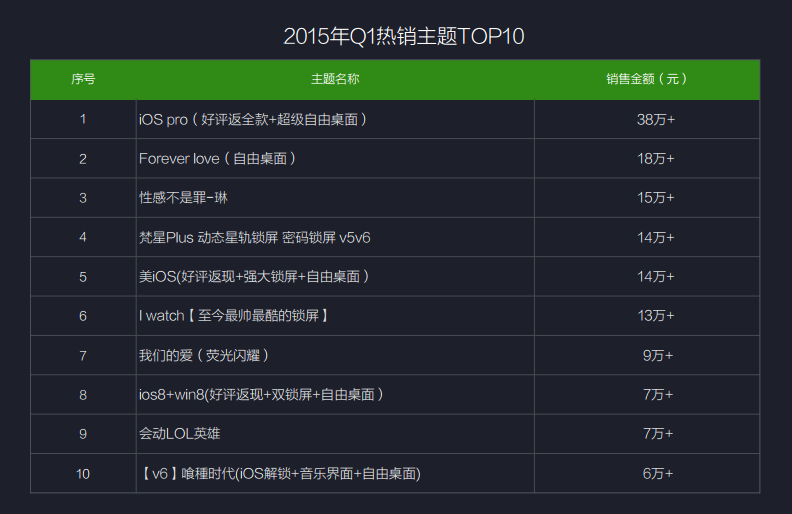
\includegraphics[scale=0.45]{figures/hl_income}}
  \figcaption{2015年Q1热销主题排行榜}
  \label{pic:hl_income}
\end{figure}

\item 支撑主题推荐系统的精准推荐。精准推荐的前提是对用户的清晰认知。以简单代金券发放为例,手机主题应用市场的历史数据呈现出两大类四种不同的消费习惯。代金券敏感型:发代金券才用、发代金券用的更多;代金券不敏感型:发不发都用,发代金券也不用。在推荐系统的用户画像系统中,上述四种群体会被分别冠以屌丝、普通、中产、土豪的标签。针对四类用户的运营策略也会全然不同,最直接的就是代金券的刺激频率以及刺激金额,而对“代金券”免疫的土豪群体,则更多地需要在优化服务上做文章。在实际场景中,影响用户对手机主题包的使用黏度的因素要远比代金券复杂得多,在这种情况下,利用用户画像可以对用户的“贴身跟踪”就能及时发现薄弱环节,因此从用户打开应用商店到退出使用,其间的每一步情况都被快的记录在案:哪一天退出的,哪一步退出的,退出之后“跳转”到什么软件等等。据此,用户画像也实现了用户另外一个纬度的归类,分清哪部分是忠实用户,哪部分可能是潜在的忠实用户,哪些则是已经流失的;更进一步来看流失的原因:因为代金券没有了流失?主题包质量不好流失?这些都是下一步精准推荐的依据。其实手机主题市场中的各项业务都与用户画像有着直接与间接的关系,无论是基于兴趣的推荐提升用户价值,精准的广告投放提升商业价值,还是针对特定用户群体的内容运营,用户画像都是其必不可少的基础支撑。直接地,用户画像可以用于兴趣匹配、关系匹配的推荐和投放;间接地,可以基于用户画像中相似的兴趣、关系及行为模式去推动用户兴趣和设计师的无缝对接。
\item 主题市场安全领域的应用。随着手机主题市场的发展,商家会通过各种活动形式的补贴来获取用户、培养用户的消费习惯,但同时也催生一些通过刷排行榜、刷红包的用户,这些行为距离欺诈只有一步之遥,但他们的存在严重破环了市场的稳定,侵占了活动的资源。其中一个有效的解决方案就是利用用户画像沉淀方法设置促销活动门槛,即通过记录用户的注册时间、历史登陆次数、常用IP地址等,最大程度上隔离掉僵尸账号,保证市场的稳定发展。
\end{itemize}

用户画像的目的是将用户信息标签化,本文介绍针对主题应用商店本身的特点介绍用户画像的构建,该用户画像主要还是从电子商务的角度出发,完善用户信息和发掘用户兴趣,区分兴趣和购买意愿,并形式化、结构化表达出来。数据的来源也主要是主题平台本身,并没有采用更多的第三方数据。

    \section{用户画像的数据来源}
    手机主题用户画像的信息来源可以有如下几种方式:
    \begin{itemize}
    \item 用户注册信息和一些评论数据。当一个新用户注册时,系统会引导用户填写一些人口基本信息,包括电话号码,性别,职业等。这些信息一般是较为可信的。当用户发生消费行为时,可能会产生购买评价和对其他用户的互动信息,这些信息是不能直接使用的,需要采用自然语言处理技术转换为较短的文本标签。
    \item 用户行为数据,包括试用,购买,浏览,点击等。不同行为代表的权重也不尽相同,试用和购买的权重高一些,浏览和点击权重低一些。
    \item 第三方应用数据。当用户注册时可用选择利用微信、微博提供的第三方免注册登陆API接口,因此这些第三方接口也可以提供一些用户信息。
    \end{itemize}

    在个性化服务的用户画像建模中,推荐系统会将以上几种方法结合起来,通过显式方式来获取静态用户信息如姓名、性别、职业等;通过隐式方式来获取动态用户信息如用户兴趣、爱好等;通过第三方登陆接口获取用户的分享、动态信息等;通过自然语言处理技术分析用户的当前心态、满意度、消费心情。

    \section{标签权重计算}
    推荐本质上是一种个性化排序,因此在收集到一个用户可能存在的标签后,还需要给标签赋一定的权重,用来区分不同标签对于该用户的重要程度。一个标签对于特定用户的权重值可以大致表示为:标签权重 = (行为类型 + 时空上下文 + 长尾因子) × 时间衰减因子。举例,用户小磊昨天购买了一款win8风格的主题包,计算公式如\autoref{tab:tagweight}所示。
    \begin{table}[htp]
    \centering
    \tabcaption{标签权重计算公式}
    \label{tab:tagweight}
    \begin{tabular}{|c|p{8cm}|} \hline
     标签 & win8风格,比较大众化,长尾因子记为 1 \\ \hline
     时间 & 昨天,衰减因子为 0.95。 \\ \hline
     行为 & 购买行为,记为权重 5 \\ \hline
     上下文 & 用户通过关键字搜索进入,最近几天有多次浏览行为,记为权重 2+2 \\ \hline
     标签权重 &  (5+1+4)*0.95=9.5 \\ \hline
    \end{tabular}
    \end{table}

    其中,用户行为类型包括浏览、添加购物车、搜索、评论、购买、点击赞、收藏等,不同的行为类型也具有不同的权重,我们定义购买权重计为5,而浏览仅仅为1。空间上下文是指用户跳转入口方式,我们定义通过搜索入口权重高于排行榜入口。时间上下文是指用户之前是否接触过此类标签,接触频率等。长尾因子是指,如果标签本身是一个非常常见的词,那么它用于刻画用户的兴趣的区分性是比较差的,相反如果是一个长尾词,则区分性较强。出于这样的考虑,越是长尾词,标签的权重值会越高。标签的权重也随着时间的流逝而变化,用户的兴趣会发生转移,时间越久远,标签的权重应该相应的下降,距离当前时间越近的兴趣标签应该得到适当突出。出于这样的考虑,一般会在标签权重值上叠加一个时间衰减函数并体现不同的时效性。此外,针对用户的兴趣,还会设定一个较小的时间窗口来获取用户的短期兴趣,短期兴趣更新周期会较长期兴趣更短,兴趣更集中,但是能够比较及时地反应用户兴趣的变化。实际生产中标签权重计算需要人工参与调整,流程如\autoref{pic:hl_abtest}
    \begin{figure}
    \centering
      \framebox{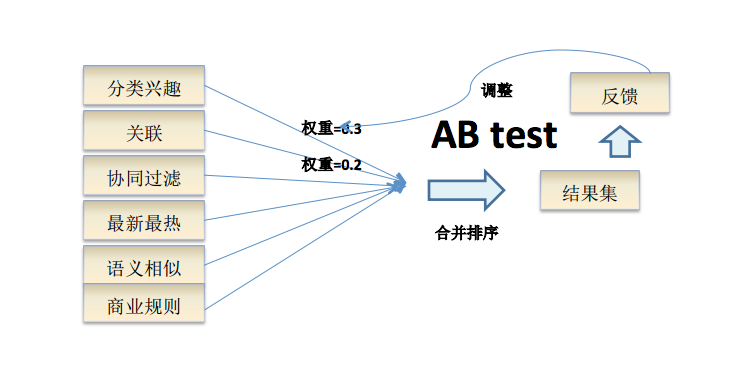
\includegraphics[scale=0.4]{figures/hl_abtest}}
      \figcaption{abtest调整标签权重}
      \label{pic:hl_abtest}
    \end{figure}

    \section{用户画像建模方式}
    根据用户在建模过程中的参与程度,用户兴趣建模采用了户手工定制建模加自动用户建模。用户手工定制建模是指用户画像由用户自己手工输入或选择的用户建模方法,如用户手工输入感兴趣信息的关键词列表,或者是选择感兴趣的栏目等。在手机主题市场早期,用户手工定制建模是用户建模的主要方法。用户手工定制建模方法实现简单、效果也不错,但它存在以下几个问题:完全依赖于用户,容易降低用户使用系统的积极性。即使用户乐意手工输入用户画像,用户也难以全面,准确的罗列自己感兴趣的栏目或关键词,导致用户标签的质量有好有坏。当用户兴趣发生变化时,用户必须重新输入用户画像,这给用户带来了额外的负担。自动用户建模是指根据用户的浏览内容和浏览行为自动构建用户画像,自动用户建模由于无需用户主动提供信息不会显示干扰用户,有利于提高个性化服务系统的亲和度,因此,自动建模是用户画像主要的建模方式。自动用户画像建模如\autoref{alg:init_userProfile}所示。
    \IncMargin{1em}
    \begin{algorithm}
      \SetKwData{Left}{left}\SetKwData{This}{this}\SetKwData{Up}{up}
      \SetKwFunction{Union}{Union}\SetKwFunction{FindCompress}{FindCompress}
      \SetKwInOut{Input}{input}\SetKwInOut{Output}{output}
      \Input{结构化用户注册信息和用户浏览行为}
      \Output{初始用户兴趣模型}
      \BlankLine
        从用户购买行为和反馈表单中提取兴趣标签及其对应的权重\\
        生成显式兴趣标签表,如{"动漫":"0.8","汽车":"0.4","美少女":"0.9"...}\\
        根据用户浏览行为获取用户兴趣标签获得隐式权重\\
        生成隐式兴趣标签表,如{"免费":"0.8","特价":"0.4","热门":"0.9"...}\\
        合并显式兴趣向量和隐式兴趣向量到当前用户画像\\
        如有新数据,返回第一步,否则跳出循环。
    \caption{自动用户画像建模算法}\label{alg:init_userProfile}
    \end{algorithm}
    \DecMargin{1em}

    \section{用户画像的维度分析}
    一个用户可以从多个方面去刻画,也就是说用户画像可以从多个维度来考虑和构建。作为虚拟电子商品交易平台,手机主题市场的用户在平台上通过某些行为(点击、浏览、购买)生产或获取信息,也通过其它一些行为(如转发、评论、赞)将信息传播出去,信息的传播是通过用户之间的社交关系所进行的,并且在生产、消费、传播信息的过程中对信息的选择和过滤体现了用户在兴趣方面的倾向性。由此,我们将用户画像按照\autoref{pic:hl_userDimension}所示的四个维度进行划分,即属性维度、兴趣维度、社交维度和行为维度。用户属性和用户兴趣是传统用户画像中包含的两个维度。前者刻画用户的静态属性特征,例如用户的身份信息(性别、年龄、受教育程度、学校等),后者则用于刻画用户在信息筛选方面的倾向(例如用户的购买能力、兴趣标签、能力标签等)。社交维度是从社交关系及信息传播的角度来刻画用户的。在社区中用户不在仅仅是一个个体,用户和用户之间的社交关系构成了一张网络,信息在这张网络中高速流动,但是这种流动并不是无差别的,信息的起始点,所经历的关键节点以及这些节点构成的关系圈都是影响信息流动的重要因素。行为维度是一个比较新的研究方向,目的是发现影响用户属性、信息变化的行为因素,分析典型用户群体的行为模式。一方面可以通过行为模式的复用来促进用户在手机主题应用平台的成长;另一方面也有利于平台认识用户,和发现新的或异常的用户行为。    
    \begin{figure}
    \centering
      \framebox{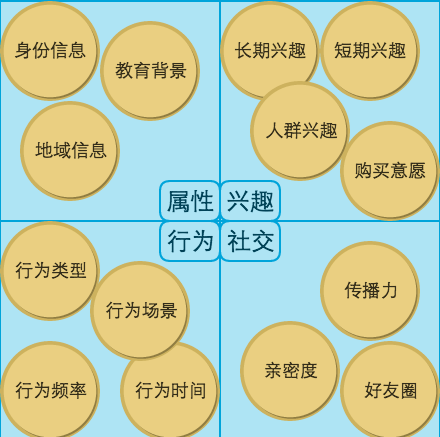
\includegraphics[scale=0.6]{figures/hl_userDimension}}
      \figcaption{用户画像维度划分}
      \label{pic:hl_userDimension}
    \end{figure}

        \subsection{属性维度}
        属性维度属于传统用户画像的范畴,即对用户的信息进行标签化。一方面,标签化是对用户信息进行结构化,方便计算机的识别和处理;另一方面,标签本身也具有准确性和非二义性,也有利于人工的整理、分析和统计。用户属性指相对静态和稳定的人口属性,包括性别、年龄区间、地域、受教育程度、学校、公司等信息的收集和建立主要依靠产品本身的引导、调查、第三方提供等,在此基础上需要进行补充和交叉验证。
        \begin{itemize}
        \item 标签来源:不是所有的词都适合充当用户标签,这些词本身应该具有区分性和非二义性;此外,还需要考虑来源的全面性,除了用户主动提供的兴趣标签外,用户在使用的过程中的行为,构建的用户关系等也能够反应用户的兴趣,因此也要将其考虑在内。
        \item 权重计算:得到了用户的兴趣标签,还需要针对用户给这些标签进行权重赋值,用来区分不同标签对于该用户的重要程度。
        \end{itemize}

        \subsection{兴趣维度}
        由于用户兴趣维度的重要性,因此有一个独立于用户画像模块的兴趣探索模块。用户兴趣是更加动态和易变化的特征,首先兴趣受到人群、环境、热点事件、行业等方面的影响,一旦这些因素发生变化,用户的兴趣容易产生迁移;其次,用户的行为多样且碎片化,不同行为反映出来的兴趣差异较大,在用户画像建模的过程中,主要考虑如下几个方面:
        \begin{itemize}
        \item 时效性:随着时间的变化,用户的兴趣会发生转移,有些兴趣会贯穿用户使用社交媒体的全过程,而有些兴趣则是受热点时间、环境因素等的影响。
        \item 长尾性:对于电商领域来讲,那些冷门的用户兴趣的总和可以和那些为数不多的大众化兴趣所占的市场份额相匹配或胜出。
        \item 兴趣和购买意愿的区分:用户具有某方面的兴趣,只代表了他愿意接受这方面的信息,并不能代表他具有购买相关内容的意愿。例如对于一些只看不买的用户,我们认为其购买意愿很小,因此对其会尽可能多的展示免费主题。
        \end{itemize}

        \subsection{社交维度}
        如果将主题应用平台的用户视作节点,用户之间的关系视作节点之间的边,那么这些节点和边将构成一个社交的网络拓扑结构,或称作社交图谱。消费信息就是在这个图谱上进行传播。从社交的维度建立用户画像,需要从不同的角度细致和全面地描述这个消费图谱的特征,反应影响信息传播的各层面上的因素,寻找节点之间的关联度,以及刻画图谱本身的结构特征。其中包括:
        \begin{itemize}
        \item 用户个体对消费信息传播的影响:不同用户在信息传播过程中的重要性不一样,影响大的用户对于信息的传播较影响小的用户更具有促进作用。
        \item 量化用户关系紧密度:存在社交关联的用户,关系越近的用户之间越容易产生相同的消费行为。
        \item 寻找相似的用户:消费中非对等的关系本身可以认为是一种认证,用户基于兴趣、消费态度等原因反应到线上的一种关联。那么在消费维度上的相似用户至少能反应他们在某种因素上的一致性。
        \item 识别关系圈:从关系图谱的本身的结构出发,从中发掘关联紧密的群体,有助于促销广告的精准投放和主题包的推广。以上关于关系建模的任务可以看作是逐步深入的,从“个体”-->“关联”-->“相似”-->“群体”的逐渐深入。
        \end{itemize}

        \subsection{行为维度}
        建立行为模式有两个任务:针对典型个体行为进行时序分片,分析用户成长的相关因素;针对典型群体的行为进行统计,为其构建通用的用户画像。
        \begin{itemize}
        \item 典型个体的行为时序分析。所谓典型个体是指某段时间内,成长比较突出的用户。例如从一个新用户从新注册到点击过百、浏览过千需要有一个积累过程,有些用户积累较快,有些较慢,而这些积累较快的用户可以作为典型个体;或者某些用户在某一阶段消费有限,但在某时刻消费激增,无论是消费金额还是数量都变化很大,这种也可以作为典型个体。针对典型个体,需要挖掘与其用户成长相关的行为因素。基本方法是对时间进行分片,获取用户在不同时间片上的行为统计,以及在各个时间分片上的用户成长指标(点击量、购买量、点击转换比等)。在此基础上针对用户行为的统计量的变化,利用关联性分析或回归来分析用户成长与哪些因素有关。
        \item 典型群体行为模式分析。针对典型个体,从用户的基本信息、人口信息、兴趣维度,可以将相似的典型用户划分为同一的群体,称作典型群体,针对典型群体中的用户按照成长程度进行划分,按不同的成长阶段统计用户行为,即建立了该典型群体的行为模型。例如,对于“年龄在20~30岁,女性,付费用户”这样的典型群体,从日点击量、月消费额等维度将其划分到初创、成长、快速提升、成熟等阶段,针对不同成长阶段内的行为组合进行统计,结果构成该群体的行为模式。如\autoref{pic:hl_usergroup}
        \end{itemize}

        \begin{figure}
        \centering
          \framebox{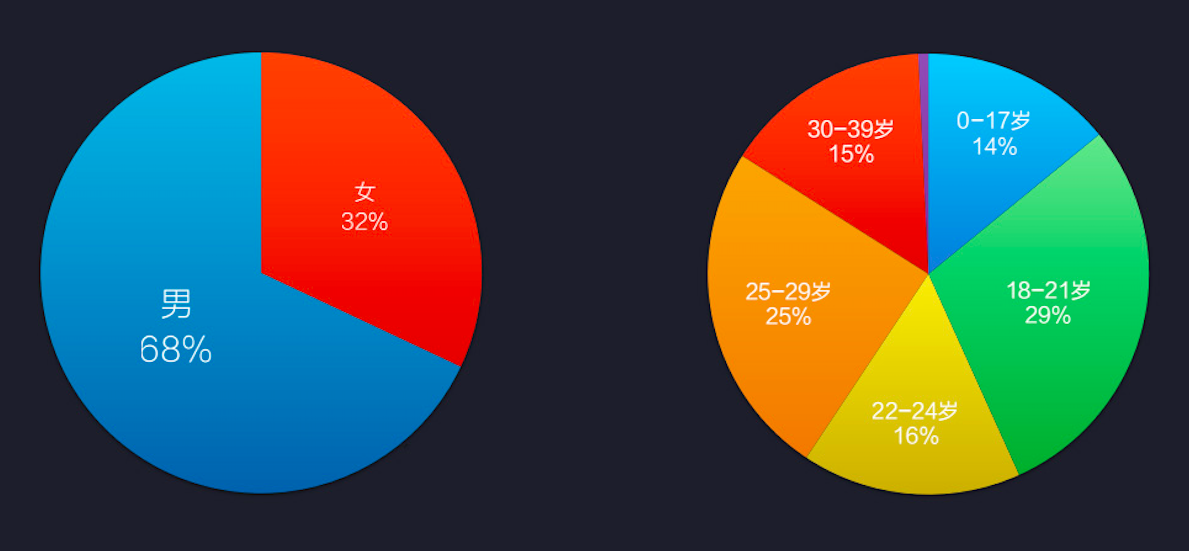
\includegraphics[scale=0.35]{figures/hl_usergroup}}
          \figcaption{手机主题市场用户群体分布}
          \label{pic:hl_usergroup}
        \end{figure}


    \section{用户画像应用场景}
      \subsection{优化手机主题市场供求}
      改变了原有的先设计、再销售的传统模式。第三方主题设计师在设计一款新产品前,会先设定好主题类型,然后通过用户画像平台中分析该用户群体的偏好,有针对性的设计产品,从而改变原先新产品高失败率的窘境,增强销售表现。如设计一款智能手表主题,面向28-35岁的年轻男性,通过在平台中进行分析,发现属性=“金属”、风格=“硬朗”、颜色=“黑色”/"深灰色"、价格区间=“中等”的偏好比重最大,那么就给新产品的设计提供了非常客观有效的决策依据。
      \subsection{提高新人留存率}
      工商管理有一个理论叫做,维护一个老用户的成本是获取新用户成本的五分之一甚至更低。所以如果能够把一些已经流失的用户召回来,这时候成本比拉一个新用户低得多,你做的事也会带来更大的价值。鉴于此公司启动了一个项目叫"用户画像之拉新",首先利用用户画像得出最近一个月没有登录过的用户数据,然后根据浏览时长分档,这是因为用户需要花自己的时间成本才能留下的最有价值的标签,之后利用用户静态标签,像姓名、职业、年龄、地域分布做进一步的细分,最后针对不同类型的用户提供不同的优惠活动。ABtest显示,与传统一刀切的推荐相比,基于用户画像的拉新留存率提高了约50\%。
      \subsection{用户消费等级分群}
      大至用户终端品牌、机型、操作系统,细至屏幕分辨率、屏幕尺寸,用户画像记录了每一个用户群体的详细终端特征。哪一类人群最容易被这款应用吸引,愿意为这款应用付费?开发者经常考虑的问题可以从用户画像找到答案。每一个用户群的价格分布、增值业务费用分布以及流量费用,包括用户详细的消费特征,比如付费频率,丰富了推荐系统的数据依据。
      \subsection{用户流失预警}
      一般情况用户在消费过程中会经历对如下几个期间:新鲜期,沉迷期,消退期,离开四个阶段,如何能够延长用户在应用的停留周期是需要解决的问题之一。用户画像可以辅助推荐系统进行流失用户特征分析,通过决策数算法,分析流失用户特征,建立不同原因流失的用户模型,然后通过这些特征得到当前在应用活跃用户中匹配流失概率高的用户数据。
      \subsection{反作弊}
      用户画像会对用户的消费能力、空闲时间、信用评级等维度进行打分;利用反作弊模型通过业务方访问收集数据,供安全部门参考。
    \section{总结}
      用户画像对于推荐系统来讲,主要如下几个方面的提升:提升推荐系统的精度,用户画像将用户的长期偏好融入到了推荐内容中,维护了推荐系统一致性。abtest显示,融合了用户画像的推荐模型比单纯的推荐模型在点击转化率指标提高了约2.8\%,考虑到300万用户的基数,2.8\%的提升是一个很大的进步;用户画像还解决新用户的冷启动问题,对于一个新注册用户来讲,推荐系统可以利用用户画像的静态信息,然后结合商品信息进行推荐;提高推荐系统的时效性,对用户行为的离线预处理,可以节约推荐系统的大部分计算时间。但是用户画像只是反映了用户长期的兴趣,所以无法动态的反映用户短期兴趣,因此我们引入了用户兴趣探索模块,将在下一章节件详细介绍。

  %自行添加
  
\chapter{用户兴趣探索}
\label{chap:interestExplore}
电子商务产品的设计往往是数据驱动的,即许多产品方面的决策都是把用户行为量化后得出的。但就商品而言,那些热门主题往往只代表了用户一小部分的个性化需求,只有通过对用户行为的充分分析,才能更好的挖掘出用户的兴趣,最终提升商品的销售量。

为了更好的探索用户兴趣,手机主题推荐系统充分利用了用户画像和商品特征表。用户画像包括基本信息和兴趣特征向量,商品特征向量表包括分类、标签、适用人群等,给定某用户行为,用户兴趣探索过程分为如下几个步骤:首先,利用用户历史行为(评论,停留时长,评分,点赞,购买等)建模量化用户满意度,然后,利用用户兴趣特征向量与商品特征向量得出相关分数,如果商品与用户的相关分数很低,但有很高的用户满意度,说明是一次成功的用户兴趣探索,更新用户画像。如果是热门商品,大量的用户都会点击,但商品与用户不是很相关,则认为其探索效果是有限的,反之如果是小众商品,考虑到长尾效应,则可以认为其是更成功的兴趣探索。这里涉及到的关键概念包括用户满意度的量化、小众标签的定向挖掘、用户兴趣的动态化。

本章内容首先介绍海量用户行为数据的存储方式。用户行为数据拥有区别于传统数据库数据的特点有,用户行为数据量巨大,常面临TB甚至PB级的数据;含有较多的噪音;多维聚合式查询。针对这些特征,用户行为数据采用Hbase数据集群存储和hadoop集群计算。然后,介绍用户兴趣探索的算法模型;然后,介绍如何通过用户行为的分析量化用户满意度。最后,介绍小众兴趣标签的挖掘。

\section{用户行为数据的存储}
手机主题用户行为数据的特点包括:用户基数庞大。手机主题注册用户达千万级,活跃用户达百万级;用户规模增长快。月新注册用户达10万数量级。每个用户的行为数量较小。即使是活跃用户,每天最多也只能产生上百条行为记录,每年不超过十万条;用户行为的计算较为复杂。计算用户的两次登录间隔天数、反复购买的商品、累积在线时间,这些都是针对用户行为的计算,通常具有一定的复杂性;用户行为数据格式不规整,字段丢失率较高。根据用户行为数据的这些特点,我们采用基于Hadop分布式的架构。Hadop又如下几个优点:
\begin{itemize}
\item 高可靠性。Hadoop按位存储和处理数据的能力使其具有高可靠性。
\item 高扩展性。Hadoop是在可用的计算机集簇间分配数据并完成计算任务的,这些集簇可以根据用户增长规模方便地扩展到数以千计的节点中。
\item 高容错性。Hadoop能够自动保存数据的多个副本,并且能够自动将失败的任务重新分配。
\item 高效性。Hadoop能够在节点之间动态地移动数据,并保证各个节点的动态平衡,因此处理速度非常快。
\item 低成本。hadoop是开源的,项目的软件成本因此会大大降低。
\end{itemize}
Hadoop的框架最核心的设计是HDFS和MapReduce。HDFS为海量的数据提供了存储,则MapReduce为海量的数据提供了计算。接下来首先介绍HDFS的体系架构,然后介绍MapReduce。
  \subsection{HDFS的体系架构}
  HDFS采用主从(Master/Slave)结构模型,一个HDFS集群是由一个NameNode和若干个DataNode组成的(在最新的Hadoop2.2版本已经实现多个NameNode的配置)。NameNode作为主服务器,管理文件系统命名空间和客户端对文件的访问操作。DataNode管理存储的数据。HDFS支持文件形式的数据。从内部来看,文件被分成若干个数据块,这若干个数据块存放在一组DataNode上。NameNode执行文件系统的命名空间,如打开、关闭、重命名文件或目录等,也负责数据块到具体DataNode的映射。DataNode负责处理文件系统客户端的文件读写,并在NameNode的统一调度下进行数据库的创建、删除和复制工作。NameNode是所有HDFS元数据的管理者,用户数据永远不会经过NameNode,HDFS体系结构图如\autoref{pic:hl_hadoop}所示。
  \begin{figure}
  \centering
    \framebox{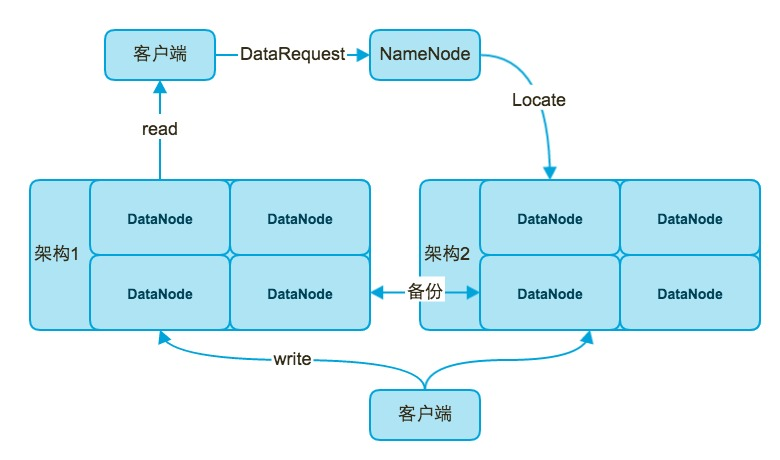
\includegraphics[scale=0.4]{figures/hl_hadoop}}
    \figcaption{HDFS体系结构}
    \label{pic:hl_hadoop}
  \end{figure}

  其中,NameNode、DataNode、Client。NameNode是管理者,DataNode是文件存储者、Client是需要获取分布式文件系统的应用程序。HDFS作为分布式文件系统在数据管理方面设计了多重容错冗余:一个Block会有三份备份,一份在NameNode指定的DateNode上,一份放在与指定的DataNode不在同一台机器的DataNode上,一根在于指定的DataNode在同一Rack上的DataNode上。备份的目的是为了数据安全,采用这种方式是为了考虑到同一Rank失败的情况,以及不同数据拷贝带来的性能的问题。
  \begin{itemize}
  \item 文件写入:首先,Client向NameNode发起文件写入的请求;然后,NameNode根据文件大小和文件块配置情况,返回给Client它管理的DataNode的信息;最后,Client将文件划分为多个block,根据DataNode的地址,按顺序将block写入DataNode块中。
  \item 文件读取:首先,Client向NameNode发起读取文件的请求;然后,NameNode返回文件存储的DataNode信息;最后,Client读取文件信息。
  \end{itemize}

  \subsection{MapReduce体系架构}
  MR框架是由一个单独运行在主节点上的JobTracker和运行在每个集群从节点上的TaskTracker共同组成。主节点负责调度构成一个作业的所有任务,这些任务分布在不同的不同的从节点上。主节点监视它们的执行情况,并重新执行之前失败的任务。从节点仅负责由主节点指派的任务。当一个Job被提交时,JobTracker接受到提交作业和配置信息之后,就会将配置信息等分发给从节点,同时调度任务并监控TaskTracker的执行。JobTracker可以运行于集群中的任意一台计算机上。TaskTracker负责执行任务,它必须运行在DataNode上,DataNode既是数据存储节点,也是计算节点。JobTracker将map任务和reduce任务分发给空闲的TaskTracker,这些任务并行运行,并监控任务运行的情况。如果JobTracker出了故障,JobTracker会把任务转交给另一个空闲的TaskTracker重新运行。

  HDFS和MR共同组成Hadoop分布式系统体系结构的核心。HDFS在集群上实现了分布式文件系统,MR在集群上实现了分布式计算和任务处理。HDFS在MR任务处理过程中提供了文件操作和存储等支持,MR在HDFS的基础上实现了任务的分发、跟踪、执行等工作,并收集结果,二者相互作用,完成分布式集群的主要任务。Hadoop上的并行应用程序开发是基于MR编程框架。MR编程模型原理:利用一个输入的key-value对集合来产生一个输出的key-value对集合。MR库通过Map和Reduce两个函数来实现这个框架。用户自定义的map函数接受一个输入的key-value对,然后产生一个中间的key-value对的集合。MR把所有具有相同的key值的value结合在一起,然后传递个reduce函数。Reduce函数接受key和相关的value结合,reduce函数合并这些value值,形成一个较小的value集合。通常我们通过一个迭代器把中间的value值提供给reduce函数,这样就可以处理无法全部放在内存中的大量的value值集合了。

  MapReduce体系中数据流动过程:首先,大数据集被分成众多小的数据集块,若干个数据集被分在集群中的一个节点进行处理并产生中间结果。然后,单节点上的任务,map函数一行行读取数据获得数据的(k1,v1),数据进入缓存,通过map函数执行map(基于key-value)排序执行后输入(k2,v2),有时候在map之后reduce之前有一个数据合并(Combine)操作,即将中间有相同的key的对合并,Combine能减少中间结果key-value对的数目,从而降低网络流量。最后,不同机器上的(k2,v2)通过merge排序的过程,reduce合并得到,(k3,v3),输出到HDFS文件中。数据流示意图如\autoref{pic:hl_MapReduce}所示。值得一提的是,Map任务的中间结果在做完Combine和Partition后,以文件的形式存于本地磁盘上。中间结果文件的位置会通知主控JobTracker,JobTracker再通知reduce任务到哪一个DataNode上去取中间结果。所有的map任务产生的中间结果均按其key值按hash函数划分成R份,R个reduce任务各自负责一段key区间。每个reduce需要向许多个map任务节点取的落在其负责的key区间内的中间结果,然后执行reduce函数,最后形成一个最终结果。有R个reduce任务,就会有R个最终结果,很多情况下这R个最终结果并不需要合并成一个最终结果,因为这R个最终结果可以作为另一个计算任务的输入,开始另一个并行计算任务。这就形成了多个输出数据片段(HDFS副本)。
  \begin{figure}
  \centering
    \framebox{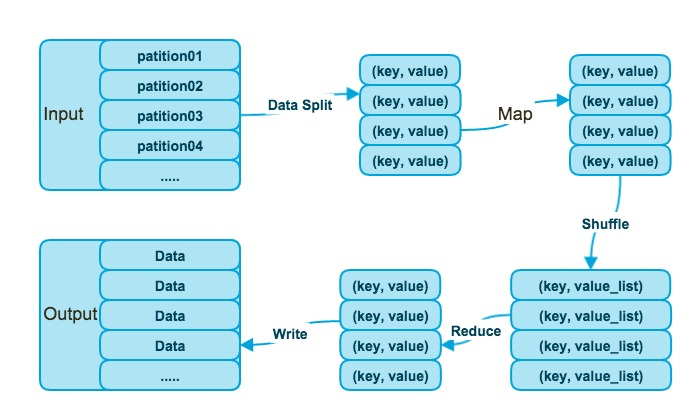
\includegraphics[scale=0.5]{figures/hl_MapReduce}}
    \figcaption{MapReduce数据流}
    \label{pic:hl_MapReduce}
  \end{figure}

  \subsection{Hbase数据管理}
  Hbase作为Hadoop数据仓库。与传统的mysql、oracle还是有很大的差别。NoSql数据库与传统关系型数据的区别有如下几个方面:
  \begin{itemize}
  \item Hbase适合大量插入同时又有读的情况。输入一个Key获取一个value或输入一些key获得一些value。
  \item Hbase的瓶颈是硬盘传输速度。Hbase的操作包括往数据里面insert数据,update的实际上也是insert,只是插入一个新的时间戳的一行。Delete数据也是insert,只是insert一行带有delete标记的一行。Hbase的所有操作都是追加插入操作。Hbase是一种日志集数据库。存储方式像是日志文件一样,是批量大量的往硬盘中写,通常都是以文件形式的读写。所以读写速度就取决于硬盘与机器之间的传输有多快。而Oracle的瓶颈是硬盘寻道时间。其经常的操作时随机读写。要update一个数据,先要在硬盘中找到这个block,然后将其读入内存,在内存中的缓存中修改,过段时间再回写回去。硬盘的寻道时间主要由转速来决定的,所以形成了寻道时间瓶颈。
  \item Hbase中数据可以保存许多不同时间戳的版本。数据按时间排序,因此Hbase特别适合寻找按照时间排序寻找Top n的场景。找出某个人最近浏览的主题,最近购买的N款主题包,N种行为等等,因此Hbase在互联网应用非常多。
  \item Hbase的局限。只能做很简单的Key-value查询。它适合有高速插入,同时又有大量读的操作场景。而这种场景又很极端,并不是每一个公司都有这种需求。在一些公司,就是普通的OLTP(联机事务处理)随机读写。在这种情况下,Oracle的可靠性,系统的负责程度又比Hbase低一些。而且Hbase局限还在于它只有主键索引,因此在建模的时候就遇到了问题。
  \item Oracle是行式数据库,而Hbase是列式数据库。列式数据库的优势在于数据分析这种场景。数据分析与传统的OLTP的区别。数据分析,经常是以某个列作为查询条件,返回的结果也经常是某一些列,不是全部的列。在这种情况下,行式数据库反应的性能就很低效。
  \end{itemize}

  \subsection{Hive数据管理}
  Hive是建立在Hadoop上的数据仓库基础架构。它提供了一系列的工具,用来进行数据提取、转换、加载,是一种可以存储、查询和分析存储在Hadoop中的大规模数据机制。可以把Hadoop下结构化数据文件映射为一张成Hive中的表,并提供类sql查询功能,除了不支持更新、索引和事务,sql其它功能都支持。可以将sql语句转换为MapReduce任务进行运行,作为sql到MapReduce的映射器。提供shell、JDBC/ODBC、Thrift等接口。优点是成本低可以通过类sql语句快速实现简单的MapReduce统计。作为一个数据仓库,Hive的数据管理按照使用层次可以从元数据存储、数据存储和数据交换三个方面介绍。
  \begin{itemize}
  \item 元数据存储。Hive将元数据存储在RDBMS中,有三种方式可以连接到数据库:1)内嵌模式:元数据保持在内嵌数据库的Derby,一般用于单元测试,只允许一个会话连接;2)多用户模式:在本地安装Mysql,把元数据放到Mysql内;3)远程模式:元数据放置在远程的Mysql数据库。
  \item 数据存储。首先,Hive没有专门的数据存储格式,也没有为数据建立索引,用于可以非常自由的组织Hive中的表,只需要在创建表的时候告诉Hive数据中的列分隔符和行分隔符,这就可以解析数据了。其次,Hive中所有的数据都存储在HDFS中,Hive中包含4中数据模型:Tabel、ExternalTable、Partition、Bucket。Table类似与传统数据库中的Table,每一个Table在Hive中都有一个相应的目录来存储数据。例如:一个表zz,它在HDFS中的路径为:/wh/zz,其中wh是在hive-site.xml中由用户设定的数据仓库的目录,所有的Table数据(不含External Table)都保存在这个目录中。Partition类似于传统数据库中划分列的索引。在Hive中,表中的一个Partition对应于表下的一个目录,所有的Partition数据都存储在对应的目录中。例如:zz表中包含ds和city两个Partition,则对应于ds=20140214,city=beijing的HDFS子目录为:/wh/zz/ds=20140214/city=Beijing;Buckets对指定列计算的hash,根据hash值切分数据,目的是为了便于并行,每一个Buckets对应一个文件。将user列分数至32个Bucket上,首先对user列的值计算hash,比如,对应hash=0的HDFS目录为:/wh/zz/ds=20140214/city=Beijing/part-00000;对应hash=20的,目录为:/wh/zz/ds=20140214/city=Beijing/part-00020。ExternalTable指向已存在HDFS中的数据,可创建Partition。和Table在元数据组织结构相同,在实际存储上有较大差异。Table创建和数据加载过程,可以用统一语句实现,实际数据被转移到数据仓库目录中,之后对数据的访问将会直接在数据仓库的目录中完成。删除表时,表中的数据和元数据都会删除。ExternalTable只有一个过程,因为加载数据和创建表是同时完成。世界数据是存储在Location后面指定的HDFS路径中的,并不会移动到数据仓库中。
  \item 数据交换。用户接口包括客户端、Web界面和数据库接口,元数据通常存储在关系数据库如Mysql,Derby中。
  \end{itemize}
本小节主要介绍了Hadoop分布式计算平台最核心的分布式文件系统HDFS、MapReduce处理过程,以及数据仓库工具Hive和分布式数据库Hbase,基本涵盖了Hadoop分布式平台的所有技术核心。从体系架构到数据定义到数据存储再到数据处理,Hadoop分布式存储、计算平台为海量用户行为的分析和用户兴趣探索提供了可能。接下来的章节先介绍用户行为数据的分析,包括数据预处理和异常数据监测,然后介绍用户兴趣探索模块,包括算法模型、用户满意度量化、小众兴趣标签的挖掘。

\section{用户行为数据的的预处理}
数据预处理是数据挖掘过程中一个重要步骤,当原始数据存在不一致、重复、含噪声、维度高等问题时,更需要进行数据的预处理,以提高数据挖掘对象的质量,最终达到提高数据挖掘所获模式知识质量的目的。
  \subsection{背景}
  随着手机主题市场交易规模的逐步增大,积累下来的业务数据和用户行为数据越来越多,这些用户数据往往是电子商务平台最宝贵的财富。目前在手机主题推荐系统中大量地应用到了机器学习和数据挖掘技术,例如个性化推荐、搜索排序、用户画像建模等等,为企业创造了巨大的价值。本节主要介绍在用户兴趣探索实践中的数据预处理与特征挖掘方法。数据预处理主要工作是:
  \begin{itemize}
  \item 从原始数据,如文本、图像或者应用数据中清洗出特征数据和标注数据
  \item 对清洗出的特征和标注数据进行处理,例如样本采样,样本调权,异常点去除,特征归一化处理等过程。最终生成的数据主要是供模型直接使用。
  \end{itemize}

  \subsection{特征提取}
  用户兴趣探索的任务包括:探索用户的兴趣广度、兴趣深度、兴趣变动趋势。依据这些信息,推荐系统就能知道在面对某一个用户时要推荐哪几类型商品,每类商品所占的比例,未来几天推荐内容会有哪些变化。在确定了目标之后,接下来需要确定使用哪些数据来达到目标。提取哪些特征数据可能与用户是否点击购买相关,一方面可以借鉴一些业务经验,另一方面可以采用一些特征选择、特征分析等方法。从业务经验来判断,可能影响用户是否点击下单的因素有:
  \begin{itemize}
  \item 用户历史行为。对于老用户,之前可能有过点击、购买等行为。
  \item 用户实时兴趣。
  \item 用户满意度。上面的特征都是比较好衡量的,用户满意度可能是更复杂的一个特征,具体体现在用户评分、评价、购买后使用频率、时长等。
  \item 是否热门,商品评价人数,购买数等。
  \end{itemize}
  在确定好要使用哪些数据之后,还需要对使用数据的可用性进行评估,包括数据的获取难度,数据的规模,数据的准确率,数据的覆盖率等。
  \begin{itemize}
  \item 用户历史行为。只有老用户才会有行为,新用户是没有的。
  \item 数据获取难度。获取用户id不难,但是获取用户年龄和性别较困难,因为用户注册或者购买时,这些并不是必填项,即使填了也不完全准确。如果一些特征需要通过其他预测模型交叉验证的话,就存在着模型精度的问题。
  \item 数据覆盖率。数据覆盖率也是一个重要的考量因素,例如地理位置特征,并不是所有用户的距离我们都能获取到,PC端的就没有地理位置,还有很多用户禁止使用它们的定位功能。
  \item 用户实时行为。如果用户刚打开app,还没有任何行为,同样面临着一个冷启动的问题。
  \item 数据的准确率。有时候用户购买一款主题,不一定是其真心喜欢,可能是因为遇到限时半价、购买返现等活动。
  \end{itemize}

  \subsection{特征获取方式}
  特征提取方式分为在线提取和离线提取。

  离线特征获取方案。离线可以使用海量的数据,借助于分布式文件存储平台,例如HDFS等,使用例如MapReduce,Spark等处理工具来处理海量的数据等。

  在线特征获取方案。在线特征比较注重获取数据的延时,由于是在线服务,需要在非常短的时间内获取到相应的数据,对查找性能要求非常高,可以将数据存储在索引、key-value存储等,也可以使用Kafka等处理工具。Kafka是一种分布式的,基于发布/订阅的消息系统。主要设计目标如下:1)以时间复杂度为O(1)的方式提供消息持久化能力,即使对TB级以上数据也能保证常数时间的访问性能;2)高吞吐率。即使在非常廉价的商用机器上也能做到单机支持每秒100K条消息的传输;3)同时支持离线数据处理和实时数据处理;4)分布式系统,易于向外扩展。所有的producer、broker和consumer都会有多个,均为分布式的。无需停机即可扩展机器。

  \subsection{用户行为数据预处理}
  根据不同业务数据的预处理方式也不同,一般来讲原始服务器日志数据脏数据的形成原因包括:缩写词不统一,数据输入错误,不同的惯用语,重复记录,丢失值,不同的计量单位,过时的编码等。相应的,数据预处理内容包括数据清理、数据异常值检测、数据集成、数据变换、数据归约、数据离散化。

  1)数据清理包括格式标准化、异常数据清除、错误纠正、重复数据的清除。对于手机主题用户数据来讲,引起空缺值的原因主要是用户设备异常造成的,有些时候是因为与其他已有数据不一致而被删除或数据的改变没有进行日志记载。根据数据空缺情况的不同有不同的处理方式:
  \begin{itemize}
  \item 忽略元组。当一个记录中有多个属性值空缺、特别是关键信息丢失时,已不能反映真实情况,它的效果非常差。
  \item 去掉属性。缺失严重时,已无挖掘意义。
  \item 人工填写空缺值。但是工作量大且可行性低。
  \item 默认值。比如使用unknown或-∞。
  \item 使用属性的平均值填充空缺值。
  \item 预测最可能的值填充空缺值。使用贝叶斯公式或判定树这样的基于推断的方法。
  \end{itemize}

  2)数据异常值就是一个测量变量中的随机错误或偏差,对于手机主题用户数据来讲,引起不正确属性值的原因包括恶意hack行为、数据输入、传输错误等。根据面临的业务不同有不同的处理方式:
  \begin{itemize}
  \item 基于统计的异常值检测。首先建立一个数据统计模型,异常是那些模型不能完美拟合的对象,对于常用的回归模型,如\autoref{pic:hl_regression}所示,异常是相对远离预测值的对象。需要注意的是,离群点是一个对象,关于数据的概率分布模型,它具有低概率。这种情况的前提是必须知道数据集服从什么分布。
  \begin{figure}
  \centering
    \framebox{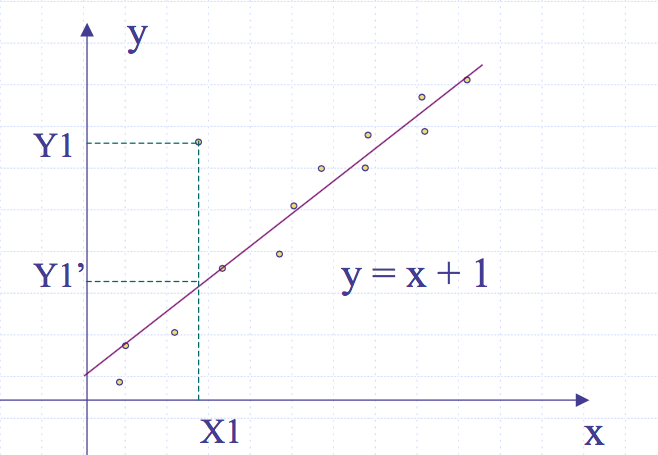
\includegraphics[scale=0.5]{figures/hl_regression}}
    \figcaption{回归异常值检测}
    \label{pic:hl_regression}
  \end{figure}
  \item 基于密度的异常值检测。离群点是在低密度区域中的对象,一个对象的离群点得分是该对象周围密度的逆。基于密度的离群点检测与基于邻近度的离群点检测密切相关,因为密度通常用邻近度定义。一种常用的定义密度的方法是,定义密度为到k个最近邻的平均距离的倒数。如果该距离小,则密度高,反之亦然。另一种密度定义是使用DBSCAN聚类算法使用的密度定义,即一个对象周围的密度等于该对象指定距离d内对象的个数。需要小心的选择d,如果d太小,则许多正常点可能具有低密度,从而具有高离群点得分。如果d太大,则许多离群点可能具有与正常点类似的密度。
  \item 基于聚类的异常值检测。如\autoref{pic:hl_cluster}所示。一种利用聚类检测离群点的方法是丢弃远离其他簇的小簇。这个方法可以和其他任何聚类技术一起使用,但是需要最小簇大小和小簇与其他簇之间距离的阈值。这种方案对簇个数的选择高度敏感。使用这个方案很难将离群点得分附加到对象上。一种更系统的方法,首先聚类所有对象,然后评估对象属于簇的程度。基于聚类的离群点:一个对象是基于聚类的离群点,如果该对象不强属于任何簇。离群点对初始聚类的影响:如果通过聚类检测离群点,则由于离群点影响聚类,存在一个问题:结构是否有效。为了处理该问题,可以使用如下方法:对象聚类,删除离群点,对象再次聚类。还有一种更复杂的方法:取一组不能很好的拟合任何簇的特殊对象,这组对象代表潜在的离群点。随着聚类过程的进展,簇在变化。不再强属于任何簇的对象被添加到潜在的离群点集合;而当前在该集合中的对象被测试,如果其现在强属于一个簇,就可以将其从潜在的离群点集合中移除。
  \begin{figure}
  \centering
    \framebox{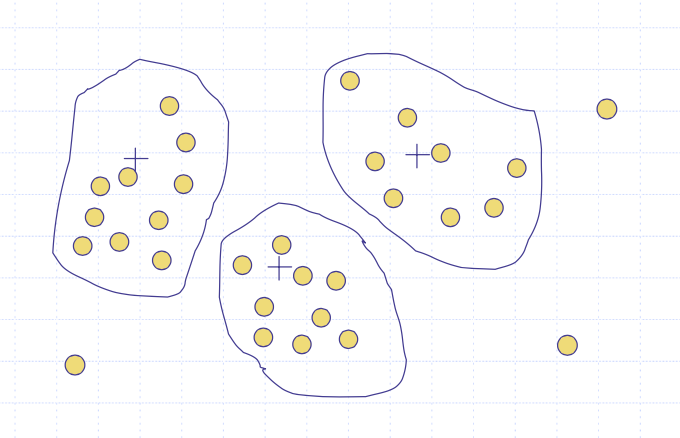
\includegraphics[scale=0.5]{figures/hl_cluster}}
    \figcaption{聚类异常值检测}
    \label{pic:hl_cluster}
  \end{figure}
  \end{itemize}

  3)数据集成就是将多个数据源中的数据整合到一个一致的存储中,需要注意以下几个情况:
  \begin{itemize}
  \item 模式集成。整合不同数据源中的元数据时的实体识别问题,比如匹配俩个表中的用户ID,A.custId=B.customerNo。
  \item 检测/解决数值冲突。对现实世界中的同一实体,来自不同数据源的属性值可能有所不同,如同表示停留时长,A表单位是秒,B表单位为毫秒。
  \item 多表之间的数据冗余。同一属性在不同的数据库中会有不同的字段名,有些时候冗余可以被相关分析检测出来,计算公式如所示,其中$\overline{A}$和$\overline{B}$表示为字段A和B的平均值,$\sigma_A和\sigma_B$表示其的标准差。仔细将多个数据源中的数据集成起来,能够减少或避免结果数据中的冗余与不一致性,从而可以提高挖掘的速度和质量。
  \begin{equation}
    r_{A,B} = \frac{\sum (A-\overline{A})(B-\overline{B})}{(n-1)\sigma_A\sigma_B}
    \label{F-Measure}
  \end{equation}
  \end{itemize}

  4)数据变换包括数据的平滑变换、数据聚集和数据规范化。所谓规范化是指将数据按比例缩放,使之落入一个小的特定区间,有如下几种方式:
  \begin{itemize}
  \item 最小-最大规范化。如\autoref{equ:minMax}所示,原始数值范围为[min,max],通过公式映射到新区间[newMin,newMax],$v'$表示属性v的公式映射。
  \begin{equation}
    v' = \frac{v-min}{max-min}(newMax-newMin)+newMin
    \label{equ:minMax}
  \end{equation}
  \item z-score规范化。Z-score表示原始数据偏离均值的距离长短,而该距离度量的标准是标准方差,如果统计数据量足够多,Z-score数据分布可以满足,68\%的数据分布在“-1”与“1”之间,95\%的数据分布在“-2”与“2”之间,99\%的数据分布在“-3”与“3之间”。如\autoref{equ:zscore}所示,其中v是原始数据,v'为v的映射,mean是全部数据的均值,$\sigma$为标准方差。
  \begin{equation}
    v' = \frac{v-mean}{\sigma}
    \label{equ:zscore}
  \end{equation}
  \item 小数定标规范化,小数定标规范化通过移动数据A的小数点位置进行规范化,小数点的移动位置依赖数据A的最大值。如\autoref{equ:small}所示,其中j是使$Max(| v'|)<1$的最小整数。
  \begin{equation}
    v' = \frac{v}{10^j}
    \label{equ:small}
  \end{equation}
  \end{itemize} 

  5)数据归约是数据字段从源数据集中得到数据集的归约表示。数据仓库中往往存有海量数据,在其上进行复杂的数据分析与挖掘需要很长的时间,通过数据归约使得数据小得多,且可以产生相同的分析结果,需要注意的是用于数据归约的时间不应当超过或“抵消”在归约后的数据上挖掘节省的时间。数据归约策略包括:
  \begin{itemize}
  \item 数据立方体聚集。最底层的方体对应于基本方体,基本方体对应于感兴趣的实体。在数据立方体中存在着不同级别的汇总,每次较高层次的抽象将进一步减少结果数据。数据立方体提供了对预计算的汇总数据的快速访问,所有尽可能对于汇总数据的查询使用数据立方体。
  \item 维归约,通过删除不相干的属性或维减少数据量,维归约又属性子集选择和启发式俩种实现方式。属性子集选择是指找出最小属性集,使得数据类的概率分布尽可能的接近使用所有属性的原分布,同时减少出现在发现模式上的属性的数目,使得模式更易于理解。启发式的方法有:逐步向前选择;逐步向后删除;向前选择和向后删除相结合;判定归纳树;基于统计分析的归约如主成分分析、回归分析等。
  \end{itemize}

  6)数据离散化,即连续属性的范围划分为区间,减少给定连续属性值的个数,区间的标号可以代替实际的数据值。
  \begin{itemize}
  \item 概念分层。通过使用高层的概念替代底层的属性值,如用青年、中年、 老年代替年龄数据值。
  \item 分箱(binning)。分箱技术递归的用于结果划分,可以产生概念分层。
  \item 直方图分析(histogram)。直方图分析方法递归的应用于每一部分,可以 自动产生多级概念分层。
  \item 聚类分析。将数据划分成簇,每个簇形成同一个概念层上的一个节点,每个簇可再分成多个子簇,形成子节点。
  \item 基于熵的离散化。
  \item 自然划分。将数值区域划分为相对一致的、易于阅读的、看上去更直观或自然的区间,划分步骤:如果一个区间最高有效位上包含3,6,7或9个不同的值,就将该区间划分为3个等宽子区间;如果一个区间最高有效位上包含2,4,或8个不 同的值,就将该区间划分为4个等宽子区间;如果一个区间最高有效位上包含1,5,或10个 不同的值,就将该区间划分为5个等宽子区间;将该规则递归的应用于每个子区间,产生给定数值属性的概念分层;对于数据集中出现的最大值和最小值的极端分布,为了避免上述方法出现的结果扭曲,可以在顶层分段时,选用一个大部分的概率空间,如5\%-95\%。
  \end{itemize}

\section{用户兴趣探索的算法模型}
用户兴趣探索就是要通过大数据挖掘建立一个用户兴趣模型,模型中包含用户的一个或更多个兴趣。首先针对本章节涉及到的对象域做出限定解释。

  \subsection{基本概念概述}
  \begin{itemize}
  \item 实体域。当我们想基于用户行为分析来建立用户兴趣模型时,我们必须把用户行为和兴趣主题限定在一个实体域上。个性化推荐落实在具体的推荐中都是在某个实体域的推荐。对于手机主题应用市场来说,实体域包括所有的主题,背景图片,铃声,闹铃等。兴趣主题。
  \item 用户行为。浏览,点击,下载,试用,购买,评论等都可是用户行为。本文所指的用户行为都是指用户在某实体域上的行为。比如用户在手机主题产生的行为。
  \item 用户兴趣。用户的兴趣维度,同样是限定在某实体域的兴趣,通常以标签+权重的形式来表示。比如,对于手机主题,用户兴趣向量可以是「动漫,0.6」,「体育,0.1」,「情感,0.7」等分类标签。值得一提的是,用户兴趣只是从用户行为中抽象出来的兴趣维度,并无统一标准。而兴趣维度的粒度也不固定,如「体育」,「电影」等一级分类,而体育下有「篮球」,「足球」等二级分类,篮球下有「NBA」,「CBA」,「火箭队」等三级分类。我们选取什么粒度的兴趣空间取决于具体用户兴趣模型。
  \item 兴趣空间。在同一层次上兴趣维度的集合,比如手机主题中,可以用「新上架」,「热门」,「特价」,「免费」来构成一个兴趣空间,也可以用「二次元」,「萝莉」,「魔幻」,「纯真」,「召唤兽」·····「法术」构成一个动漫兴趣空间。
  \end{itemize}
用户满意度的量化;小众兴趣标签的挖掘;动态兴趣;然后提出一种分布式的大规模并行聚类算法,并将该算法应用到该三部图模型中;基于浏览内容的兴趣度模型[7-8]、基于用户浏览行为的兴趣度模型[9]和动态变化的用户兴趣模型

  
\chapter{动态推荐系统设计}
  \section{前言}
  推荐系统的形式化定义如下:设C是所有用户的集合,S是所有可以推荐给用户的主题的集合。实际上,C和S集合的规模通常很大,如上百万的顾客以及上亿种歌曲等。设效用函数u()可以计算主题s对用户c的推荐度(如提供商的可靠性(vendorreliability)和产品的可得性(productavailability)等),即$u=C\times S \rightarrow R$,R是一定范围内的全序的非负实数,推荐要研究的问题就是找到推荐度R最大的那些主题S*,如\autoref{equ:fromal}
    \begin{equation}
    \forall c \in C,S^{*}=arg  max_{s \in S} u(c,s)
    \label{equ:fromal}
    \end{equation}
  除了推荐系统自身如冷启动、数据的稀疏性等问题,还有一个关注点就是推荐系统的时间效应问题。比较常见的时间效应问题主要反映在用户兴趣的变化、物品流行度的变化以及商品的季节效应,这些问题都可以利用用户画像解决。本章节主要介绍如何搭建一个具有长尾性、实时性的动态推荐形态。动态推荐形态由3个重要的模块组成:用户画像、兴趣探索模块、推荐主题建模模块、推荐算法模块和评测指标模块。通用的推荐系统模型流程如所示。推荐系统把用户模型中兴趣需求信息和推荐主题模型中的特征信息匹配,同时使用相应的推荐算法进行计算筛选,找到用户可能感兴趣的推荐主题,然后推荐给用户。

  用户画像模块对应着用户长期兴趣,用户兴趣探索对应着用户短期动态兴趣。短期兴趣的特点是临时、易变;长期兴趣的特点是长久、稳定;用户的短期兴趣可能会转化为长期兴趣,所以需要在推荐时综合考虑长期兴趣和短期兴趣。考虑到推荐系统的时间效应问题,将输入数据集归结为一个四元组,即{用户,物品,行为,时间},通过研究用户的历史行为来预测用户将来的行为。需要解决以下俩个问题:动态评分预测、时效性的影响。首先,动态评分预测问题。数据集可以选用比较直观的显性反馈数据集,即(用户,物品,评分,时间),研究是这样一个问题,给定用户u,物品i,时间t,预测用户u在时间t对物品i的评分r。对于该类问题,与时间无关的评分预测问题算法主要有以下几种:用户兴趣的变化,如年龄增长,从儿童长成青少年壮年;生活状态的变化,由以前的小学生到大学生;社会事件的影响如俩会等。此外还有季节效应问题,一些在春季很流行的,在夏季节未必就很流行。该问题的解决有待进一步思考。对于时效性的影响,每个在线系统都是一个动态系统,但它们有不同的演化速率。比如说,新闻,手机主题更新很快,但音乐,电影的系统演化的却比较慢。

  本章首先介绍用户画像和兴趣探索模块,其中兴趣探索模块需要根据业务的演化速率来调整迭代深度。然后介绍推荐主题模块,之后介绍推荐算法模块和指标体系,最后做总结。
  
  \section{用户画像和兴趣探索模块}
  目前基于用户画像的推荐,主要用在基于内容的推荐,从最近的RecSys大会(ACM Recommender Systems)上来看,不少公司和研究者也在尝试基于用户画像做Context-Aware的推荐(情境感知,又称上下文感知)。利用用户的画像,结合时间、天气等上下文信息,给用户做一些更加精准化的推荐是一个不错的方向。一个好的推荐系统要给用户提供个性化的、高效的、动态准确的推荐,那么推荐系统应能够获取反映用户多方面的、动态变化的兴趣偏好,推荐系统有必要为用户建立一个用户兴趣探索模型,该模型能获取、表示、存储和修改用户兴趣偏好,能进行推理,对用户进行分类和识别,帮助系统更好地理解用户特征和类别。推荐系统根据用户画像进行推荐,所以用户画像对推荐系统的质量有至关重要的影响。建立用户画像模型之前,需要考虑:模型的输入数据有哪些,如何获取模型的输入数据;如何考虑用户的兴趣及需求的变化;建模的对象是谁以及如何建模;模型的输出是什么。用户画像模型的输入数据主要有以下几种:
  \begin{itemize}
  \item 用户属性,分为社会属性和自然属性,包括用户最基本的如用户的姓名、年龄、职业、收入、学历等信息。用户注册时的对自然属性和社会属性进行初始建模。 
  \item 用户手工输入的信息:是用户主动输出给系统的信息,包括用户在搜索引擎中打出的关键词,用户评论中发布的感兴趣的主题、频道。还有一类重要的信息就是用户反馈的信息,包括用户自己对推荐结果的满意程度;用户标注的浏览页面的感兴趣、不感兴趣或感兴趣的程度等。
  \item 用户的浏览行为和浏览内容:用户浏览的行为和内容体现了用户的兴趣和需求,它们包括浏览次数、频率、停留时间等,浏览页面时的操作(收藏、保存、复制等)、浏览时用户表情的变化等。服务器端保存的日志也能较好地记录用户的浏览行为和内容。
  \item 推荐对象的属性特征:不同的推荐对象,用户建模的输入数据也不同。网页等推荐对象通常考虑对象的内容和用户之间的相似性,而产品等推荐对象通常考虑用户对产品的评价。为提高推荐质量,推荐对象的相关的属性也要考虑进去,比如除网页内容以外,还要考虑网页的发布人、时间等。产品类的对象还要考虑产品的品牌、价格、出售时间等。
  \end{itemize}

  用户行为的权重排序。用户显式行为数据记录了用户在平台上不同的环节的各种行为,这些行为一方面用于候选集触发算法中的离线计算(主要是点击、浏览),另外一方面,这些行为代表的用户兴趣强弱不同,因此在训练重排序模型时可以针对不同的行为设定不同的权重值,以更细地刻画用户的行为强弱程度。此外,用户的购买、试用等行为还可以作为重排序模型的交叉特征,用于模型的离线训练和在线预测。负反馈数据反映了当前的结果可能在某些方面不能满足用户的需求,因此在后续的候选集触发过程中需要考虑对特定的因素进行过滤或者降权,提高用户体验;同时在重排序的模型训练中,A/B测试结果可以作为不可多得的负例参与模型训练。用户画像是刻画用户属性的元数据,其中有些是直接获取的基础数据,有些是经过挖掘的二次数据,这些属性一方面可以用于候选集触发过程中对标签进行加权或降权,另外一方面可以作为重排序模型中的用户维度特征。通过对数据的挖掘可以提取出一些关键词,然后使用这些关键词给主题打标签,用于主题的个性化展示。

  用户行为的获取方式。模型输入数据的方式有显式获取、隐式获取和启发式获取三种方式。显式获取用户兴趣偏好的方法是简单而直接的做法,能准确地反映用户的需求,同时所得的信息比较具体、全面、客观,结果比较可靠。缺点就是数量稀少,原因用户不太愿意花时间来向商家表达自己的喜好,并且这种方法灵活性差,答案存在异质性,当用户兴趣主题改变时需要用户手动更改系统中用户兴趣。同时该方法对用户不是很人性化。解决人性化问题是推荐系统未来的一个研究方向,来研究用户能够接受的评价方式是什么,比如能够有耐心进行几次评分。利用固定负担模型来计量用户评价的负担,将人性化设计问题转化为最优化问题来研究。隐式获取法是指系统通过记录用户行为数据,通过权重排序获取用户的兴趣偏好,用户的很多动作都能暗示用户的喜好,包括查询、浏览页面和文章、标记书签、反馈信息、滑屏等。隐式的跟踪可以在建立用户画像基本数据的同时不打扰用户的正常消费活动。这种方法的缺点就是跟踪的结果未必能正确反映用户的兴趣偏好。同时系统若过度跟踪用户的历史记录,有时会引发用户隐私问题,而放弃对当前推荐系统的使用。 上述获取兴趣偏好的方法有时受用户教育背景、职业和习惯等因素的限制,用户有时意识不到自己的兴趣主题,因此能为用户提供启发式信息,如领域术语抽取和相似度物品聚类,可以实现领域知识的复用,为用户间的协同提供支持,提高用户兴趣获取质量。用户的兴趣和需求会随着时间和情景发生变化,用户画像模块要考虑到用户长期兴趣偏好和短期兴趣偏好,还要考虑兴趣的变化,目前很多研究关注了用户的长期兴趣,建立了静态用户画像模型,但用户兴趣探索模型也越来越受到关注。结合长期和短期兴趣的动态建模将是未来的一个研究方向,如\autoref{pic:hl_iterate}所示。
  \begin{figure}
    \centering
      \framebox{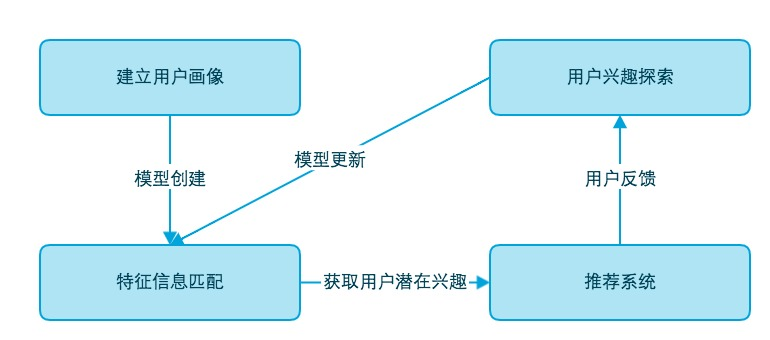
\includegraphics[scale=0.4]{figures/hl_iterate}}
      \figcaption{用户画像的使用}
      \label{pic:hl_iterate}
  \end{figure}

  用户画像更新采用了时间窗方法和遗忘机制来反映用户兴趣的变化。目前的更新机制无法及时跟踪用户兴趣的变化,just-in-time型有更强学习效率和动态变化适应能力的建模也是未来的重要研究方向。 

  \section{推荐主题模块}
  推荐主题分为单用户建模和群组建模,单用户建模针对个体用户进行建模,比如基于主题内容的推荐,群组建模是针对一类用户进行建模,比如基于商品的协同推荐。

  应用于不同的领域的推荐系统其推荐的主题也各不相同,如何对推荐主题进行描述对推荐系统也有很重要的影响。和用户画像一样,要对推荐主题进行描述之前要考虑:提取推荐主题的什么特征,如何提取,提取的特征用于什么目的,主题的特征描述和用户画像之间有关联。提取到的每个主题特征标签对推荐结果会有什么影响。主题的特征描述文件能否自动更新。
  推荐主题的描述文件中的主题特征和用户画像中的兴趣标签进行推荐计算,获得推荐主题的推荐权重,所以推荐主题的描述文件与用户画像密切相关,通常的做法是用同样的方法来表达用户的兴趣偏好和推荐主题。推荐系统推荐主题包括众多的领域,比如体育、动漫、科技、国家,还有诸如音乐、电影等多媒体资源等等。不同的主题,特征也不相同,目前并没有一个统一的标准来进行统一描述,主要有基于内容的方法和基于分类的方法两大类方法。 基于内容的方法是从主题本身抽取相关信息来表示主题,使用最广泛的方法是用加权关键词矢量,该方法通过对标注主题的标签进行统计分析得出的特征向量。方法很多,比较简单的做法就是计算每个特征的熵,选取具有最大熵值的若干个特征;也可以计算每个标签的信息增量(Information gain),即计算每个特征在主题中出现前后的信息熵之差;还可以计算每个特征的互信息(mutual information),即计算每个特征和主题的相关性。在完成主题特征提取后,还需要计算每个特征的权值,权值大的对推荐结果的影响就大。基于分类的方法是把推荐主题放入不同类别中,这样可以把同类主题推荐给对该类主题感兴趣的用户了。文本分类的方法有多种,比如朴素贝叶斯(Naive-Bayes),k最近邻方法(KNN)和支持向量机(SVM)等。 主题的类型可以预先定义,也可以利用聚类算法自动产生。研究表明聚类的精度非常依赖于主题的数量,而且由自动聚类产生的类型可能对用户来说是毫无意义的,因此可以有选择的进行手工选定的类型来分类主题,在没有对应的候选类型或需要进一步划分某类型时,才使用聚类产生的类型。推荐系统推荐给用户的主题首先不能与用户购买过的主题重复,其次也不能与用户刚刚看过的主题不是太形似或者太不相关,这就是所谓的模型过拟合问题(可扩展性问题)。出现这一问题的本质上来自数据的不完备性,解决的主要的方法是引入随机性,使算法收敛到全局最优或者逼近全局最优。针对这一问题考察了被推荐的主题的相关性和冗余性,要同时保证推荐的多样性,又不能与用户看过的主题重复或毫不相关。关于这一问题的研究是推荐系统研究的一个难点和重点。 推荐系统中出现新的主题时,推荐系统尤其是协同过滤系统中,新主题出现后必须等待一段时间才会有用户浏览和评价,而在此之前推荐系统是无法对此主题进行推荐,这就是推荐系统研究的另一个难点和重点——商品冷启动问题。解决这一问题的方法就是考虑利用组合推荐方法。
  
  \section{推荐算法模块}
  推荐算法类型很多,但是各有各的局限,比较常用的有基于内容推荐,协同过滤推荐,基于关联规则推荐,基于效用推荐,基于知识推荐,组合推荐。他们的主要优缺点对比如所示。
  \begin{table}[htp]
  \centering
  \tabcaption{推荐系统主要算法比较}
  \label{tab:algarithm}
  \begin{tabular}{ |c|p{6cm}|p{6cm}| } \hline
   推荐方法 & 优点 & 缺点 \\ \hline
   基于内容推荐 & 推荐结果直观,容易解释;不需要领域知识 & 稀疏问题;新用户问题;复杂属性不好处理;要有足够数据构造分类器 \\ \hline
   协同过滤推荐 & 新异兴趣发现、不需要领域知识;随着时间推移性能提高;推荐个性化、自动化程度高;能处理复杂的非结构化对象 & 稀疏问题;可扩展性问题;新用户问题;质量取决于历史数据集;系统开始时推荐质量差; \\ \hline
   基于规则推荐 & 能发现新兴趣点;不要领域知识 & 规则抽取难、耗时;产品名同义性问题;个性化程度低; \\ \hline
   基于效用推荐 & 无冷开始和稀疏问题;对用户偏好变化敏感;能考虑非产品特性 & 用户必须输入效用函数;推荐是静态的,灵活性差;属性重叠问题; \\ \hline
   基于知识推荐 & 能把用户需求映射到产品上;能考虑非产品属性 & 知识难获得;推荐是静态的\\ \hline
  \end{tabular}
  \end{table}
  推荐算法本身是一个综合性的问题,可以简单地用最基本的Content-based,再复杂点可以Collaborative Filtering,更深入一些诸如基于SVD/LDA等的降维算法和基于SVD++等的评分预测算法,或者把推荐问题再转换成分类问题,或者采用以上算法前先用各种聚类算法做数据的预处理。
    
    \subsection{推荐算法}
    基于内容推荐。基于内容的推荐(Content-based Recommendation)是信息过滤技术的延续与发展,它是建立在项目的内容信息上作出推荐的,而不需要依据用户对项目的评价意见,更多地需要用机 器学习的方法从关于内容的特征描述的事例中得到用户的兴趣资料。在基于内容的推荐系统中,项目或对象是通过相关的特征的属性来定义,系统基于用户评价对象 的特征,学习用户的兴趣,考察用户资料与待预测项目的相匹配程度。用户的资料模型取决于所用学习方法,常用的有决策树、神经网络和基于向量的表示方法等。 基于内容的用户资料是需要有用户的历史数据,用户资料模型可能随着用户的偏好改变而发生变化。基于内容推荐方法的优点是:不需要其它用户的数据,没有冷开始问题和稀疏问题。能为具有特殊兴趣爱好的用户进行推荐。能推荐新的或不是很流行的项目,没有新项目问题。通过列出推荐项目的内容特征,可以解释为什么推荐那些项目。已有比较好的技术,如关于分类学习方面的技术已相当成熟。缺点是要求内容能容易抽取成有意义的特征,要求特征内容有良好的结构性,并且用户的口味必须能够用内容特征形式来表达,不能显式地得到其它用户的判断情况。

    协同过滤推荐。协同过滤推荐(Collaborative Filtering Recommendation)技术是推荐系统中应用最早和最为成功的技术之一。它一般采用最近邻技术,利用用户的历史喜好信息计算用户之间的距离,然后 利用目标用户的最近邻居用户对商品评价的加权评价值来预测目标用户对特定商品的喜好程度,系统从而根据这一喜好程度来对目标用户进行推荐。协同过滤最大优 点是对推荐对象没有特殊的要求,能处理非结构化的复杂对象,如音乐、电影。协同过滤是基于这样的假设:为一用户找到他真正感兴趣的内容的好方法是首先找到与此用户有相似兴趣的其他用户,然后将他们感兴趣的内容推荐给此用户。其基本 思想非常易于理解,在日常生活中,我们往往会利用好朋友的推荐来进行一些选择。协同过滤正是把这一思想运用到电子商务推荐系统中来,基于其他用户对某一内 容的评价来向目标用户进行推荐。基于协同过滤的推荐系统可以说是从用户的角度来进行相应推荐的,而且是自动的,即用户获得的推荐是系统从购买模式或浏览行为等隐式获得的,不需要用户努力地找到适合自己兴趣的推荐信息,如填写一些调查表格等。和基于内容的过滤方法相比,协同过滤具有如下的优点:能够过滤难以进行机器自动内容分析的信息,如艺术品,音乐等。共享其他人的经验,避免了内容分析的不完全和不精确,并且能够基于一些复杂的,难以表述的概念(如信息质量、个人品味)进行过滤。有推荐新信息的能力。可以发现内容上完全不相似的信息,用户对推荐信息的内容事先是预料不到的。这也是协同过滤和基于内容的过滤一个较大的差别,基于内容的过滤推荐很多都是用户本来就熟悉的内容,而协同过滤可以发现用户潜在的但自己尚未发现的兴趣偏好。能够有效的使用其他相似用户的反馈信息,较少用户的反馈量,加快个性化学习的速度。 虽然协同过滤作为一种典型的推荐技术有其相当的应用,但协同过滤仍有许多的问题需要解决。最典型的问题有稀疏问题(Sparsity)和可扩展问题(Scalability)。协同过滤(CF)可以看做是一个分类问题,也可以看做是矩阵分解问题。协同滤波主要是基于每个人自己的喜好都类似这一特征,它不依赖于个人的基本信息。比如刚刚那个电影评分的例子中,预测那些没有被评分的电影的分数只依赖于已经打分的那些分数,并不需要去学习那些电影的特征。

    基于关联规则推荐。基于关联规则的推荐(Association Rule-based Recommendation)是以关联规则为基础,把已购商品作为规则头,规则体为推荐对象。关联规则挖掘可以发现不同商品在销售过程中的相关性,在零 售业中已经得到了成功的应用。管理规则就是在一个交易数据库中统计购买了商品集X的交易中有多大比例的交易同时购买了商品集Y,其直观的意义就是用户在购 买某些商品的时候有多大倾向去购买另外一些商品。比如购买牛奶的同时很多人会同时购买面包。算法的第一步关联规则的发现最为关键且最耗时,是算法的瓶颈,但可以离线进行。其次,商品名称的同义性问题也是关联规则的一个难点。

    基于效用推荐。基于效用的推荐(Utility-based Recommendation)是建立在对用户使用项目的效用情况上计算的,其核心问题是怎么样为每一个用户去创建一个效用函数,因此,用户资料模型很大 程度上是由系统所采用的效用函数决定的。基于效用推荐的好处是它能把非产品的属性,如提供商的可靠性(Vendor Reliability)和产品的可得性(Product Availability)等考虑到效用计算中。

    基于知识推荐。基于知识的推荐(Knowledge-based Recommendation)在某种程度是可以看成是一种推理(Inference)技术,它不是建立在用户需要和偏好基础上推荐的。基于知识的方法因它们所用的功能知识不同而有明显区别。效用知识(Functional Knowledge)是一种关于一个项目如何满足某一特定用户的知识,因此能解释需要和推荐的关系,所以用户资料可以是任何能支持推理的知识结构,它可以是用户已经规范化的查询,也可以是一个更详细的用户需要的表示。

    组合推荐。由于各种推荐方法都有优缺点,所以在实际中,组合推荐(Hybrid Recommendation)经常被采用。研究和应用最多的是内容推荐和协同过滤推荐的组合。最简单的做法就是分别用基于内容的方法和协同过滤推荐方法 去产生一个推荐预测结果,然后用某方法组合其结果。尽管从理论上有很多种推荐组合方法,但在某一具体问题中并不见得都有效,组合推荐一个最重要原则就是通 过组合后要能避免或弥补各自推荐技术的弱点。在组合方式上,有研究人员提出了七种组合思路:加权(Weight):加权多种推荐技术结果。变换(Switch):根据问题背景和实际情况或要求决定变换采用不同的推荐技术。混合(Mixed):同时采用多种推荐技术给出多种推荐结果为用户提供参考。特征组合(Feature combination):组合来自不同推荐数据源的特征被另一种推荐算法所采用。层叠(Cascade):先用一种推荐技术产生一种粗糙的推荐结果,第二种推荐技术在此推荐结果的基础上进一步作出更精确的推荐。特征扩充(Feature augmentation):一种技术产生附加的特征信息嵌入到另一种推荐技术的特征输入中。元级别(Meta-level):用一种推荐方法产生的模型作为另一种推荐方法的输入。

    \subsection{AB测试}
    产品的改变并不总是意味着进步,有时候无法评判多种设计方案中哪一种更优秀的, 这时A/B测试就派上用场了,A/B测试可以回答两个问题:哪个方案好结果的可信程度A/B测试结果是基于用户得到的结果,用数据说话, 而不是凭空想象去为用户代言,并且通过一定的数学分析给出结果的可信度。A/B测试需要如下几个前提:多个方案并行测试;每个方案只有一个变量不同;能够以某种规则优胜劣汰其中第2点暗示了A/B测试的应用范围:A/B测试必须是单变量,但有的时候,我们并不追求知道某个细节对方案的影响,而只想知道方案的整体效果如何,那么可以适当增加变量,当然测试方案有非常大的差异时一般不太适合做A/B测试,因为它们的变量太多了,变量之间会有很多的干扰,所以很难通过A/B测试的方法找出各个变量对结果的影响程度。在满足上述前提时,便可以做A/B测试了。

    目标转换率变化区间估计:在做A/B测试的时候,抽样得到的数据并不能准确反映整体的真实水平,即样本得到的估计是有偏差的,因此需要去评估这个值可能的变化区间。例如通过区间估计得到:A方案转换率为:6.5\% ± 1.5\%B方案转换率为:7.5\% ± 1.5\%方案胜出概率估计:由于最终有意义的是确立胜出的版本,然而并不是所有的实验都能做到样本足够大,区分度足够高的,因此确定版本胜出的概率,很多英文资料里面记为Chance to beat baseline,即在给定转换率下,变体版本的实际转换率高于参展版本(默认是原始版本)的实际转换率的可能性。在实验之前需要设定一个阈值(称为置信度),某版本胜出的可能性高于这个值并且稳定时,便可以宣布该版本胜出。置信度越高,结果的可靠信越高;随着置信度的增加实验时间将会变长。

  \section{动态推荐系统底层架构}
    \subsection{基于Spark}
    基于Spark的方式在架构上,第一种是使用Spark把模型计算放在内存中,加快模型计算速度,Hadoop中作业的中间输出结果是放到硬盘的HDFS中,而Spark是直接保存在内存中,因此Spark能更好地适用于数据挖掘与机器学习等需要迭代的模型计算,如表9-2所示。
    \begin{table}[htp]
    \centering
    \tabcaption{MR和spark对比}
    \label{tab:spark}
    \begin{tabular}{ |p{3cm}|p{5cm}|p{5cm}| } \hline
     过程 & MapReduce & Spark \\ \hline
     collect & 在内存中构造了一块数据结构用于map输出的缓冲 & 没有在内存中构造一块数据结构用于map输出的缓冲,而是直接把输出写到磁盘文件 \\ \hline
     sort & map输出的数据有排序 & map输出的数据没有排序 \\ \hline
     merge & 对磁盘上的多个spill文件最后进行合并成一个输出文件 & 在map端没有merge过程,在输出时直接是对应一个reduce的数据写到一个文件中,这些文件同时存在并发写,最后不需要合并成一个 \\ \hline
     copy框架 & jetty & netty或者直接socket流 \\ \hline
     对于本节点上的文件 & 仍然是通过网络框架拖取数据 & 不通过网络框架,对于在本节点上的map输出文件,采用本地读取的方式\\ \hline
     copy过来的数据存放位置 & 先放在内存,内存放不下时写到磁盘 & 一种方式全部放在内存;另一种方式先放在内存\\ \hline
     merge sort & 最后会对磁盘文件和内存中的数据进行合并排序 & 对于采用另一种方式时也会有合并排序的过程\\ \hline
    \end{tabular}
    \end{table}

    \subsection{基于Kiji框架}
    Kiji是一个用来构建大数据应用和实时推荐系统的开源框架,本质上是对HBase上层的一个封装,用Avro来承载对象化的数据,使得用户能更容易地用HBase管理结构化的数据,使得用户姓名、地址等基础信息和点击、购买等动态信息都能存储到一行,在传统数据库中,往往需要建立多张表,在计算的时候要关联多张表,影响实时性。Kiji提供了一个KijiScoring模块,它可以定义数据的过期策略,如综合产品点击次数和上次的点击时间,设置数据的过期策略把数据刷新到KijiScoring服务器中,并且根据自己定义的规则,决定是否需要重新计算得分。如用户有上千万浏览记录,一次的行为不会影响多少总体得分,不需要重新计算,但如果用户仅有几次浏览记录,一次的行为,可能就要重新训练模型。Kiji也提供了一个Kiji模型库,使得改进的模型部署到生产环境时不用停掉应用程序,让开发者可以轻松更新其底层的模型。

    \subsection{基于Storm}
    最后一种基于 Storm 的实时推荐系统。在动态推荐上,算法本身不能设计的太复杂,手机主题推荐系统的数据库是TB级别,实时读写大表比较耗时。可以把算法分成离线部分和实时部分,利用Hadoop离线任务尽量把查询数据库比较多的、可以预先计算的模型先训练好,或者把计算的中间数据先计算好,比如,线性分类器的参数、聚类算法的群集位置或者协同过滤中条目的相似性矩阵,然后把少量更新的计算留给Storm实时计算,一般是具体的评分阶段。用HBase或HDFS存储历史的浏览、购买行为信息,用Hadoop基于User CF的协同过滤,先把用户的相似度离线生成好,用户到商品的矩阵往往比较大,运算比较耗时,把耗时的运行先离线计算好,实时调用离线的结果进行轻量级的计算有助于提高主题推荐的实时性。协同过滤算法在storm上计算过程为:首先程序获取用户和主题的历史数据,得到用户到主题的偏好矩阵,利用Jaccard相似系数(Jaccard coefficient)、向量空间余弦相似度(Cosine similarity)、皮尔逊相关系数(Pearson correlation coefficient)等相似度计算方法,得到相邻的用户(User CF)或相似商品(Item CF)。在User CF中,基于用户历史偏好的相似度得到邻居用户,将邻居用户偏好的主题推荐给该用户;在Item CF中,基于用户对物品的偏好向量得到相似主题,然后把这款主题推荐给喜欢相似主题的其他用户。然后通过Kafka或者Redis队列,保存前端的最新浏览等事件流,在Storm的Topology中实时读取里面的信息,同时获取缓存中用户topN个邻居用户,把邻居用户喜欢的商品存到缓存中,前端从缓存中取出商品,根据一定的策略,组装成推荐列表。除了相似性矩阵,其他模型大体实现也相似,比如实际的全品类电商中不同的品类和栏位,往往要求不同的推荐算法,如母婴主题,如果结合商品之间的序列模式和母婴年龄段的序列模式,效果会比较好,可以把模型通过Hadoop预先生成好,然后通过Storm实时计算来预测用户会买哪些主题。

  \section{量化评估推荐系统}
  推荐系统还是看目的是如何的,从用户角度讲是为了更好的理解用户,减少用户查找内容的时间和次数,从产品本身角度讲,是增加单位面积单位时间内的点击数或者说内容有效。 从业务角度的衡量:衡量点击和打开率,这说明用户是否对内容感兴趣。衡量通过推荐系统替代用户主动搜索或者主动浏览的次数,可以通过横向与使用其他产品对比较,比如使用推荐系统提供内容的用户搜索次数和点击浏览目录次数明显下降。衡量推荐系统的满意度口碑,刨除因为页面位置效果等因素,衡量推荐系统一个重要的就是满意度的口碑问题,这个可以通过单个用户是否有重复使用的行为,曲线是否是一直上升的来衡量,如果一直有新用户访问,但一直没有老用户重复使用,说明用户满意度有问题。
  \section{总结}
  推荐系统经过了相当时间的发展,同时一些重点和难点问题得到了研究者的关注,相信是未来研究的热点问题。用户兴趣偏好获取方法和推荐对象的特征提取方法的研究目前的推荐系统中实际上较少使用了用户和推荐对象的特征,即使使用很广泛的协同推荐使用的是用户的评分。主要是用户兴趣偏好的获取方法和推荐对象特征提取方法不是很适用,需要引入更精确适用的用户和对象特征。(2)推荐系统的安全性研究进行协同推荐时需要掌握用户的兴趣偏好等用户信息,但用户担心个人数据得不到有效保护而不愿暴露个人信息,这是协同推荐长期存在的一个问题。既能得到用户信息而提高推荐系统性能,又能有效保护用户信息将是未来推荐系统的一个研究方向。同时一些不法的用户为了提高或降低某些对象的推荐概率,恶意捏造用户评分数据而达到目的,这也是推荐系统存在的一个安全问题,被称为推荐攻击[93-96]。检测并能预防推荐攻击也将是未来一个研究方向。(3)基于复杂网络理论及图方法的推荐系统研究复杂网络理论和图方法同协同推荐存在契合点,在文献中网络视频推荐问题转化为热量散播平衡态网络上的谱图分割问题,通过设计长尾发现的推荐策略引导用户发现潜在的感兴趣的网络视频。利用复杂网络理论和图方法进行推荐也是推荐系统研究的一个方向。(4)推荐的多维度研究目前的推荐研究都是基于用户-对象二维空间进行研究的,但是用户选择某个对象以及对对象的评分在不同的情况下会有所不同,也就是推荐使用的特征维度会有所不同,研究推荐的多维度也是未来的一个研究方向。(5)稀疏性和冷启动研究稀疏性和冷启动问题是困扰推荐系统很长时间了,包括经典协同过滤算法和新出现的基于网络结构的推荐算法都存在该问题。有很多研究者对这一问题进行研究并提出解决办法,但该问题依然存在,还需要对其进行研究。(6)推荐系统性能评价指标的研究用户对算法准确度的敏感度、算法对不同领域的普适性、广义的质量评价方法等都是未来推荐系统性能评价要进行研究的目标。

%%%%%%%%%%%%%%%%%%%%%%%%%%%%%%
%% 附件部分
%%%%%%%%%%%%%%%%%%%%%%%%%%%%%%
\backmatter

  % 参考文献
  % 使用 BibTeX
  % 选择参考文献的排版格式。注意ustcbib这个格式不保证完全符合要求,请自行决定是否使用
  %\bibliographystyle{ustcbib}%{GBT7714-2005NLang-UTF8}
 % \bibliography{bib/tex}
  %\nocite{*} % for every item
  % 不使用 BibTeX
  %\renewcommand{\baselinestretch}{0.5}
\begin{thebibliography}{10}

\bibitem{recmd-youtube}
Shumeet Baluja, Rohan Seth, D. Sivakumar, Yushi Jing, Jay Yagnik, Shankar Kumar, Deepak Ravichandran, and Mohamed Aly.2008.
\newblock {\em Video sug- gestion and discovery for youtube: taking random walks through the view graph}.
\newblock In Proceeding of the 17th international conference on World Wide Web, WWW ’08, pages 895–904.

\bibitem{recmd-system}
Francesco Ricci and Lior Rokach and Bracha Shapira.2011.
\newblock {\em Introduction to Recommender Systems Handbook[M]}.
\newblock Springer, 1-35. 

\bibitem{recmd-netflix}
Robert M. Bell and Yehuda Koren. December 2007.
\newblock {\em Lessons from the netflix prize challenge}.
\newblock SIGKDD Explor. Newsl., 9:75–79.

\bibitem{demo-data}
Bruce Krulwich.1997.
\newblock {\em Lifestyle finder: Intelligent user profiling using large-scale demographic data[C]}.
\newblock AI Magazine, 18(2):37–45.

\bibitem{cognitive-science}
Elaine Rich.1998.
\newblock {\em Readings in intelligent user interfaces[C]}.
\newblock chapter User modeling via stereotypes, 329–342. 

\bibitem{Forecast-principle}
J. Scott Armstrong, editor.2001.
\newblock {\em Principles of Forecasting - A Handbook for Researchers and Practitioners[M]}.
\newblock Kluwer Academic.

\bibitem{cf-sn}
Henry Kautz, Bart Selman, and Mehul Shah. March 1997.
\newblock {\em Referral web: combining social networks and collaborative filtering[C]}.
\newblock Commun. ACM, 40:63–65.

\bibitem{Amazon-cf}
Greg Linden, Brent Smith, and Jeremy York. January 2003.
\newblock {\em Amazon.com recommendation- s: Item-to-item collaborative filtering[C]}.
\newblock IEEE Internet Computing, 7:76–80.

\bibitem{info-overload}
Anne-F. Rutkowski and Carol S. Saunders.June 2010.
\newblock {\em Growing pains with information overload[C]}.
\newblock Computer, 43:96–95.

\bibitem{info-overload:1}
Anne-F. Rutkowski and Carol S. Saunders.June 2010.
\newblock {\em Growing pains with information overload[C]}.
\newblock Computer, 43:96–95.

\bibitem{recmd-history}
Liu, Yu; Li, Weijia; Yao, Yuan; Fang, Jing; Ma, Ruixin; Yan, Zhaofa.
\newblock {\em An Infrastructure for Personalized Service System Based on Web2.0 and Data Mining}.
\newblock International Conference on Intelligent Computing and Information Science. JAN 08-09, 2011.

\bibitem{user-interest}
Sia K.C, Zhu S.Chi, Hino Tseng, B.L.2006.
\newblock {\em Capturing User Interests by Both Exploitation and Exploration[C]}.
\newblock Technical report, NEC Labs America. 

\bibitem{recmd-xiangliang}
项亮. 2012.
\newblock {\em 推荐系统实践}.
\newblock 图灵原创,人民邮电出版社, 36:5–21.

\bibitem{content-based}
K Yoshii.2006.
\newblock {\em Hybrid Collaborative and Content-Based Music Recommendation Using Probabilistic Model with Latent User Preferences [C]}.
\newblock In: Proceedings of the International Conference on Music Information Retrieval.

\bibitem{collab-filter}
Jonathan L. Herlocker, Joseph A. Konstan, Loren G. Terveen, and John T. Riedl.January 2004.
\newblock {\em Evaluating collaborative filtering recommender systems[C]}.
\newblock ACM Trans.Inf.Syst, 22:5–53.

\bibitem{social-filter}
Henry Kautz, Bart Selman, and Mehul Shah.March 1997.
\newblock {\em Referral web: combining social networks and collaborative filtering[C]}.
\newblock Commun. ACM, 40:63–65.

\bibitem{cold-start}
Andrew I.Schein, Alexandrin Popescul, Lyle H.Ungar, David M.Pennock. 2002.
\newblock {\em Methods and Metrics for Cold-Start Recommendations[C]}.
\newblock New York City, New York: ACM. 253–260.

\bibitem{latent-cf}
Thomas Hofmann and Jan Puzicha.1999. 
\newblock {\em Latent class models for collaborative filtering[J]}.
\newblock In Proceedings of the Sixteenth International Joint Conference on Artificial Intelligence, IJCAI ’99,San Francisco, CA, USA, Morgan Kaufmann Publishers Inc, pages 688–693, 

\bibitem{date-mining}
Han Jiawei, Kamber, Micheline.2001.
\newblock {\em Data mining: concepts and techniques[C]}.
\newblock Morgan Kaufmann. 5.

\bibitem{info-retrieval}
Jansen B.J and Rieh S.2010.
\newblock {\em The Seventeen Theoretical Constructs of Information Searching and Information Retrieval[J]}.
\newblock Journal of the American Society for Information Sciences and Technology. 61(8)

\bibitem{long-tail}
O Celma. 2010.
\newblock{\em Music Recommendation and Discovery in the Long Tail[C]}.
\newblock Springer. 

\bibitem{temporal-cf}
Yehuda Koren.2009.
\newblock {\em Collaborative filtering with temporal dynamics[J]}.
\newblock In Proceedings of the 15th ACM SIGKDD international conference on Knowledge discovery and data mining, KDD ’09,New York, NY, USA., pages 447–456.

\bibitem{recmd-kmeans}
Hartigan, J.A.Wong, M.A.Algorithm.
\newblock {\em A k-Means Clustering Algorithm}.
\newblock Journal of the Royal Statistical Society, Series C. 1979, 28 (1): 100–108.

\bibitem{recmd-slopone}
Daniel Lemire, Anna Maclachlan.
\newblock {\em Slope One Predictors for Online Rating-Based Collaborative Filtering}.
\newblock In SIAM Data Mining (SDM'05), Newport Beach, California, April 21-23, 2005.

\bibitem{ab-test}
Kohavi, Ron, Longbotham, Roger.2015.
\newblock {\em Online Controlled Experiments and A/B Tests[C]}.
\newblock In Sammut.



\bibitem{recmd-Hybrid}
Robin Burke. November 2002.
\newblock {\em Hybrid recommender systems: Survey and experiments}.
\newblock User Modeling and User-Adapted Interaction, 12:331–370.

\bibitem{Personalization1}
Gediminas Adomavicius and Alexander Tuzhilin. 1999.
\newblock {\em User Profiling in Personalization Applications through Rule Discovery and Validation}.
\newblock ACM, 377-381.

\bibitem{Personalization2}
lbrahim Cingil, Asuman Dogac and Ayca Azgin.2000.
\newblock {\em A broader approach to personalization}.
\newblock mmunications of the ACM, 43(8): 136-141.

\bibitem{Personalization3}
Joseph Kramer, Sunil Noronha and John Vergo.2000.
\newblock {\em A user-centered design approach to personalization}.
\newblock Communications of the ACM, 43(8)44-48.

\bibitem{Personalization4}
Bamshad Mobasher, Honghua Dai, Tao Luo, Yuqing Sun and Jiang Zhu.2000.
\newblock {\em Integrating Web Usage and Content Mining for More Effective Personalization}.
\newblock Electronic Commerce and Web Technologies, 1875: 165-176.

\bibitem{Personalization5}
Bamshad Mobasher, Robert Cooley and Jaideep Srivastava.2000.
\newblock {\em Automatic personalization based on Web usage mining}.
\newblock Communications of the ACM, 43(8): 142-151.

\bibitem{Personalization6}
P. Chen, H. Xie, S. Maslov, and S. Redner.2007.
\newblock {\em Finding Scientific Gems with Google's PageRank Algorithm}.
\newblock Journal of Informetrics, 1(1):8--15.

\bibitem{Personalization7}
C. Basu, H. Hirsh, and W. Cohen.1998.
\newblock {\em Recommendation as Classification: Using Social and Content-Based Information in Recommendation}.
\newblock In Proc. of the 15th National Conference on Artificial Intelligence (AAAI ’98), 714–720.

\bibitem{Personalization8}
J. Teevan and S. T. Dumais and E. Horvitz.2005.
\newblock {\em Personalizing Search via Automated Analysis of Interests and Activities}.
\newblock . In Proc. of the 28th Annual International ACM SIGIR Conference on Research and Development in Information Retrieval (SIGIR 2005), 449–456,

\bibitem{Personalization9}
S. M. McNee, I. Albert, D. Cosley, S. L. P. Gopalkrishnan, A. M.Rashid, J. S. Konstan, and J. Riedl.2002.
\newblock {\em Predicting User Interests from Contextual Information}.
\newblock  In Proc. of the 2002 ACM Conference on Computer Supported Cooperative Work (CSCW ’02), 116–125,
\end{thebibliography}


  % 附录,没有请注释掉
  %\begin{appendix}
  %  
\chapter{中国科学技术大学研究生学位论文撰写规范}
\label{chap:requires}
\section*{以下文字仅作示例,一切以学校规定为准!}
研究生院规定在此下载\url{http://gradschool.ustc.edu.cn/ylb/material/xw/wdxz/1.doc}

研究生学位论文集中反映研究生在研究工作中所取得的成果,代表研究生研究工作的水平,也是申请和授予相应学位的主要依据。为提高研究生学位论文的撰写质量,做到学位论文在内容和格式上的规范化,我们编写了《中国科学技术大学研究生学位论文撰写规范》,供申请学位的研究生参考执行。其中参考文献著录规则我们根据GB/T 7714-2005的标准撰写。硕士和博士学位论文除在研究深度等方面要求不同外,撰写要求基本一致。

\section{内容要求}

\subsection{封面} 
采用研究生院规定的统一封面,封面包含内容如下: 
\subsubsection{密级} 涉密论文必须在论文封面标注密级(内部、秘密、机密),同时注明保密年限。
\subsubsection{论文题目} 应准确概括整个论文的核心内容,简明扼要,最多不超过30字,必要时可以加副标题。
\subsubsection{作者姓名} 英文封面中按英文习惯书写,即名在前。姓名需写全拼。
\subsubsection{学科专业} 写所在专业的全称,不可用简写。
\subsubsection{导师姓名} 一般允许有两名指导教师,主要指导教师姓名写在第一位,后附其职称,次要指导教师排第二位,也需注明职称。
\subsubsection{完成时间} 填写论文打印成文的年月日。

\subsection{中国科学技术大学学位论文原创性和授权使用声明}
本部分内容使用统一的模版,具体内容见格式范例,提交时作者须亲笔签名。

\subsection{摘要和关键词}
\subsubsection{中文摘要}
摘要是论文内容的总结概括,应简要说明论文的研究目的、基本研究内容、研究方法、创新性成果及其理论与实际意义,突出论文的创新之处。不宜使用公式、图表,不标注引用文献。 
\subsubsection{中文关键词} 
关键词是为了文献标引工作从论文中选取出来用以表示全文主题内容信息的单词和术语,一般3--8个词,要求能够准确概括论文的核心内容。
\subsubsection{英文摘要与关键词}
以中文书写的论文,内容与中文摘要和关键词完全一致,其他语种书写的论文以简略为原则,不需要相同。

\subsection{目录}
目录页由论文的章、条、附录等序号、名称和页码组成。论文中如图表较多,可以分别列出清单置于目次页之后。图的清单应有序号、图题和页码。表的清单应有序号、表题和页码。

\subsection{符号说明}
如果论文中使用了大量的物理量符号、标志、缩略词、专门计量单位、自定义名词和术语等,应编写成注释说明汇集表。若上述符号等使用数量不多,可以不设此部分,但必须在论文中出现时加以说明。

\subsection{正文}
正文是学位论文的主体,包括绪论、论文主体及结论等部分。
\subsubsection{绪论}
内容应包括:选题的背景和意义,文献综述及研究现状,研究内容与预期结果,研究方法和实验设计,论文结构安排等。要求实事求是,不夸大、缩小前人的工作和自己的工作,言简意赅,突出重点,不与摘要雷同。
\subsubsection{论文主体}
论文主体是正文的核心部分,占主要篇幅,它是将学习、研究和调查过程中筛选、观察和测试所获得的材料,经过加工整理和分析研究,由材料而形成论点。由于各学科及具体选题的差异,此部分不作统一规定。但总体内容必须实事求是,客观真切,准确完备,合乎逻辑,层次分明,简练可读。
\subsubsection{结论}
结论是对整个论文主要成果的总结,应明确、精炼、完整、准确。其中应明确指出本研究的创新点,对论文的学术价值和应用价值等加以预测和评价,说明研究中尚难解决的问题并提出今后进一步在本研究方向进行研究工作的设想或建议。

\subsection{参考文献}
本着以严谨求实的科学态度撰写论文,凡学位论文中有引用或参考、借用他人成果之处,均应详细列出所引文献的名称、作者、发表刊物、发表时间、卷号、页码等,严禁抄袭剽窃。  
\subsection{附录}
主要列入正文内过分冗长的公式推导,供查读方便所需的辅助性数学工具或表格,重复性数据图表,论文使用的缩写,程序全文及说明等。

\subsection{致谢}
对给予各类资助、指导和协助完成研究工作以及提供各种对论文工作有利条件的单位及个人表示感谢。致谢应实事求是,切忌浮夸与庸俗之词。

\subsection{在读期间发表的学术论文与取得的其他研究成果}
按学术论文发表的时间顺序,列齐本人在攻读学位期间发表或已录用的学术论文清单(发表刊物名称、卷册号、页码、年月及论文署名、作者排序)。其他研究成果可以是申请的专利、获得的奖项及完成的项目等。
 
\section{书写规定}

\subsection{论文的字数要求}
硕士学位论文要求不少于3万字,博士学位论文要求不少于5万字。

\subsection{文字、标点符号和数字}
除留学生和外语专业研究生外,学位论文一律用汉字书写。除非特殊需要,不得使用已废除的繁体字、异体字等不规范汉字。标点符号的用法以GB/T 15834—1995《标点符号用法》为准。数字用法以GB/T 15835—1995《出版物上数字用法的规定》为准。

留学生的学位论文所采用语种可以和导师商定,但论文封面须用中文。

\subsection{封面与扉页}
\subsubsection{秘级} 封面的秘级可以标注为内部、秘密和机密,各密级的保密时限分别为小于等于5年、小于等于10年和小于等于20年,非保密论文不标注密级。
\subsubsection{题目} 题目中避免使用缩略词、首字母缩写字、字符、代号和公式等。
\subsubsection{日期} 封面的日期用汉字书写。
\subsubsection{扉页} 扉页的内容与封面一致。扉页后,需给出英文的封面。其他语种书写的论文还需在英文封面后附上正文所用语种书写的封面。

\subsection{目录}
目录应包括论文的全部内容,包括中英文摘要和附录等,正文章节题名要求编到第3级标题,即×.×.×。一级标题顶格书写,二级标题缩进一个汉字符位置,三级标题缩进两个汉字符位置。

\subsection{摘要与关键词}
\subsubsection{摘要}
摘要分中文和英文两种,中文在前,英文在后。标题摘要二字中间空一格。摘要的字数,硕士学位论文建议1000字以内,博士学位论文建议3000字以内。留学生用其他语种撰写学位论文时,中文摘要应不少于6000汉字。摘要中不得出现图片、图表、表格或其他插图材料。英文摘要与中文摘要应完全一致。
\subsubsection{关键词}
关键词以显著的字符另起一行并隔行排列于摘要下方,左顶格。中文关键词间空一格,英文关键词间用逗号隔开。

\subsection{论文正文}
\subsubsection{章节及各章标题}
论文正文分章节撰写,每章应另起一页。

各章标题字数一般应在15字以内,不使用标点符号。标题中尽量不采用英文缩写词,对必须采用者,应使用本行业的通用缩写词。
\subsubsection{序号}
\paragraph{标题序号}
论文标题分层设序。层次以少为宜,根据实际需要选择。各层次标题一律用阿拉伯数字连续编号;不同层次的数字之间用小圆点“.”相隔,末位数字后面不加点号,如“1”,“1.1”,“1.1.1”等;各层次的序号均左起顶格排,后空1个字距接排标题。例如:

第1章 ××××(大标题) 

1.1 ××××(一级节标题)

1.1.1 ××××(二级节标题)

1.1.1.1 ××××(根据需要,也可设三级节标题)

第2章 ××××(大标题)

2.1 ××××(一级节标题)

2.1.1 ××××(二级节标题)

\paragraph{图表等编号} 
论文中的图、表、附注、公式、算式等,一律用阿拉伯数字分章依序连续编码。其标注形式应便于互相区别,如:图 l.1(第1章第一个图)、图2.2(第二章第二个图);表3.2(第三章第二个表)等。
\paragraph{页码}
页码从绪论开始按阿拉伯数字(1,2,3……)连续编排,此前的部分(中英文摘要、目录等)用大写罗马数字(I,II,III…)单独编排,页码位置居于页脚居中。封面、扉页、创新性声明等不编页码。
\subsubsection{页眉}
页眉从中文摘要开始,内容与该部分的一级标题相同,奇偶页相同,各部分的首页也需有页眉。
\subsubsection{名词和术语}
科技名词术语及设备、元件的名称,应采用国家标准或部颁标准中规定的术语或名称。标准中未规定的术语要采用行业通用术语或名称。全文名词术语必须统一。一些特殊名词或新名词应在适当位置加以说明或注解。

采用英语缩写词时,除本行业广泛应用的通用缩写词外,文中第一次出现的缩写词应该用括号注明英文原词。
\subsubsection{量和单位}
量和单位要严格执行GB 3100~3102-93(国家技术监督局1993-12-27发布,1994-07-01实施)有关量和单位的规定。

量的符号一般为单个拉丁字母或希腊字母,并一律采用斜体(pH例外)。为区别不同情况,可在量符号上附加角标。 

在表达量值时,在公式、图、表和文字叙述中,一律使用单位的国际符号,且无例外地用正体。单位符号与数值间要留适当间隙。具体可参见下列表达式3.1。

\subsubsection{图和表}
\paragraph{图}
图应具有“自明性”,即只看图、图题和图例,不阅读正文,就可理解图意。每一图应有简短确切的题名,连同图号置于图下。

图的位置在相关说明文字之后,随文排。坐标比例不宜过大,同一图上不同曲线的点要分别用不同形状的标识符标出。图中的术语、符号、单位等应与正文表述中所用一致。

图题应简明。图号和图题间空1个字符位置,居中排于图的下方。

必要时,应将图上的符号、标记、代码,以及实验条件等,用最简练的文字,横排于图题下方,作为图例说明(图注)。

\paragraph{表}
表的位置也在相应说明文字之后,随文排。表中参数应标明量和单位的符号。表应有自明性。每一表应有简短确切的题名,连同表号置于表上,表号与表题间空一个字符位置。表号用阿拉伯数字分章编号,如第3章第2个表的表号表示为“表3.2”。

表格太大需要转页时,需要在续表上方注明“续表”,表头也应重复排出。

必要时应将表中的符号、标记、代码,以及需要说明事项,以最简练的文字,横排于表题下,作为表注。相关要求同于图注。

\subsubsection{表达式}
表达式主要指数字表达式,也包括文字表达式。表达式需另行起排,原则上应居中,用阿拉伯数字分章编号。序号加圆括号,右顶格排。例如,第3章第1个表达式:

较长的式如必须转行,只能在+,-,×,÷,<,>处转行,序号编于最后一行的最右边。

\subsection{参考文献}
参考文献参照GB/T 7714-2005《文后参考文献著录规则》执行。推荐使用著者-出版年制,即在正文引用文献处标注著者姓名与出版年份,在文后的参考文献表中标注参考文献的详细信息。
\subsubsection{著者-出版年制在正文中的标注方式}

正文中的标注方式分两种:其一,正文里已出现著作者姓名的,在其后用圆括号附上出版年份即可;其二,正文里仅提及有关的资料内容而未提到著作者,则在相应文句处用圆括号标注著作者姓名和出版年份,两者之间加逗号。

例如:

Park et al(1995)根据Laurentia西缘放射状基性岩墙的研究以及与地幔柱有关的澳大利亚Gairdner岩墙群的研究,首次提出约780Ma地幔柱导致Rodinia超大陆的裂解。

其中关于成冰系顶底界时限和冰川活动年龄、超大陆裂解的起始时间和持续时间……是当前中国地球科学界十分活跃并得到迅速发展的研究领域(王平,2003)。

引用同一著者在同一年份出版的多篇文献时,在出版年份之后用英文小写字母a、b、c……区别。如:(王平,2005a);(王平,2005b)

多处引用同一著者的同一文献时,在“()”外以角标的形式著录引文页码。引用有两个以上同姓的著者的外文文献时,则著者要加名字的缩写,但不必加缩写点。

引用多位著者的文献时,对欧美著者只需标注第一个著者的姓,其后附“et al”,仅两位作者的也可全部注出,中间用“and”;对中国著者应该标注第一著者的姓名,其后附“等”字,姓名与“等”字之间留1个空格。例如:……(王平 等,2005) ……。

同一处引用多篇文献时,按出版年份由近及远依次标注,中间用逗号分开。

\subsubsection{著者-出版年制参考文献表的编排}
 参考文献表加居中标题——“参考文献”,并列入全书目录。

凡正文里括注了著者姓名和年份的,其文献都必须列入参考文献表。

参考文献表中的条目(不排序号),先按语种分类排列,语种顺序是:中文、日文、英文、俄文、其他文种。然后,中文和日文按第一著者的姓氏笔画排序,中文也可按汉语拼音字母顺序排列,西文和俄文按第一著者姓氏首字母顺序排列。

在参考文献中,当一个著者有多篇文献并为第一著作者时,他单独署名的文献排在前面(并按出版年份的先后排列),接着排他与其他人合写的文献。

著录项目与GB/T 7714-2005《文后参考文献著录规则》中规定的顺序编码制基本相同,不同的仅为出版年份排于编著者之后。
\subsubsection{参考文献标注的注意事项}
编著者姓名,一律姓在前、名字在后。西文和俄文的姓全部著录,名字可用大写首字母(不加缩写点);如果姓和名的首字母相同,便要用全名。

以机构和团体署名的文献,此机构或团体可作为编著者,但要用全称,而不用简称或缩写。

编著者不明的文献,编著者一项应注明“佚名”,或用其他与之相应的词。 

编著者为3人以下时全部著录,用逗号分隔,3人以上可只著录前3人,后加“,等”,外文用“,et al”,“et al”不必用斜体。

外文文献大写字母的使用要符合文种本身的习惯用法。

外文期刊刊名可列出全名,也可列惯用缩写刊名(缩写点可加,也可不加,但全文要统一)。只有一个词的刊名不能缩写。期刊名排正体。

期刊只列出卷号,不必标“卷”或“Vol”等;如果是分卷图书,则应加“卷”或“册”或“Vol”或其他语种相应的词(外文缩写词不加缩写点,首字母大小写应全文统一)。

参考文献的版次、卷、期、页码等数字一律用阿拉伯数字表示。版次中中文版次著录为“第2版”、“第3版”……(第1版不必列出),西文文献的版次著录为“2nd ed”、“3rd ed”或其他语种相应的词 。

出版年采用公元纪年,并用阿拉伯数字著录。如有其他纪年形式时,将原有的纪年形式置于“( )”内。

如:1947(民国三十六年)

日文文献中的汉字要用日文汉字。

参考文献中使用的标点符号:

,用于多著者姓名之间,出版者和年或卷(期)之间,期刊名和年或卷之间,“等”或“译”字、专利号等之前。

:用于副题名之前、出版地之后,或引文页码、析出文献页码、专利国别前。

()用于期号、报纸的版次、电子文献更新或修改日期以及非公元纪年。

[] 用于序号、文献类型、电子文献的引用日期以及自拟的的信息。

∥用于专著中的析出文献的出处项前。

- 用于起讫序号和起讫页码间。

. 用于其余各项目之后。

\subsubsection{顺序编码制的著录规则}
参考文献如果按照顺序编码制著录,可参照GB/T 7714-2005《文后参考文献著录规则》执行。


\section{排版和印刷要求}略

\chapter{关于规范本科毕业论文(设计)格式和统一封面的通知}
\section*{以下文字仅作示例,一切以学校规定为准!}
教务处规定在此下载\url{http://202.38.70.92/bklw.doc}

\hspace{-2em}各院系:

鉴于目前各院系本科毕业论文(设计)存在着论文格式不够规范、封面不统一的状况,为加强本科毕业论文的管理,提高论文质量,同时规范全校本科毕业论文(设计)格式,现对本科毕业论文格式和统一封面规定如下:
\begin{enumerate}
\item 本科毕业论文按编排顺序应包括以下内容:封面、扉页、致谢、目录、中文内容摘要、英文内容摘要、正文章节、参考文献或资料注释、附录等。
\item 本科毕业论文的格式要求:
\begin{enumerate}
\item 封面中“论文题目”等内容用四号宋体。
\item 除封面、扉页外,每面上部加页眉,用小5号字标注“中国科学技术大学本科毕业论文”,居中。
\item 从目录页开始在每面底部居中用小五宋体连续编页码。
\item 论文的“致谢”、“目录”等标题用小二号黑体字,居中。
\item 目录一般列三级,后附规范的页号。
\item 正文中的标题分章、节、段三级;章、节标题居中,段标题居左,分别用三号黑体、小三黑体、四号黑体。
\item 具体内容用小四号宋体,每行间距为22磅,科学公式和符号要符合国标,公式要单独占行、居中、行距为单倍行距。
\item 表格、插图全文要分别统一编号或按章编号,标题用小四宋体:(表格标题居表上方,插图标题居图下方),居中。
\item 参考文献的内容包括:序号、作者名、书名或文章名、刊物名或出版社名、
刊物期卷、页和日期,用小四宋体,外文期刊名用白斜体。
\item 附录为:
\begin{enumerate}
\item 重要参考文献中相关内容和章节复印件;
\item 作者或导师所做的与本论文有关的成果复印件。
要求用A4纸复印附于参考文献后。
\end{enumerate}
\end{enumerate}
\item 本科毕业论文(设计)封面学校已统一印制,请到教材科领购。
\item 装订要求:每份论文必须用A4纸打印(复印)、装订成册(教材科可提供复印、装订业务)。另外,校级优秀毕业论文必须提交一份线装毕业论文交档案馆收藏。
\item 具体格式详见附件式样。
\end{enumerate}
\begin{flushright}
中国科技大学教务处

二OO二年三月二十八日
\end{flushright}
附件:本科毕业论文(设计)式样

(略)

  %\end{appendix}

  \makeatletter
  \ifustc@bachelor\relax\else
    % 致谢
	
\begin{thanks}

人生就是一个关于成长的漫长故事。而在中科大求学作为本人人生体验的一部分,亦是这样的一段故事。在此的俩年半,俯仰之间,科大的“问道”、“学术”于此,让我经历了这样的三段成长:学于师友,安于爱好,观于内心。

“古之学者必有师,师者,所以传道、授业、解惑也”。师友的教诲不可能一直跟着自己,可是他们治学态度却融入了我的人生观。授课的华保健老师的严谨、郭燕老师的认真、丁菁老师的直率、席菁老师的踏实都曾触动我,并给予我前进方向上的指引。

本论文内容为数据挖掘在电商行业的工程实现,因此有一段真实的、贴近数据挖掘领域的实习经历尤为重要。感谢我在苏州国云数据公司实习的 CEO 马晓东学长,让我有机会一窥大数据行业的内幕;感谢我在小米实习的导师方流博士,感谢我在滴滴出行工作的机器学习研究院李佩博士,让我成为大数据挖掘工程师的梦想又更近了一步;感谢我的导师周武旸教授和张四海教授,指导我完成论文。
向师友和书籍学习,是从外界汲取;只有回归到自己的内心和思绪才能沉淀.在每个夜幕深沉或是晨曦初露的时刻里,感受自己情绪的流动,反思自己的取舍得失,然后才有了融于师友和书籍时的奋进。这样的三段成长,如今已是一体,不断地相互印证与反馈!

“逝者如斯夫,不舍昼夜”。成长亦复如是,不断的和昨日的自己告别。但是,一路有你,真好!相会是缘,同行是乐,共事是福!

\vskip 18pt

\begin{flushright}

~~~~\ustc@author~~~~

\today

\end{flushright}

\end{thanks}
%硕博致谢部分
    % 发表文章目录
    %\include{chapter/pub}
  \fi
  \makeatother

\end{document}
